Some published numerical experiments have over time become benchmarks for other codes, while some 
others showcased comparisons between codes. Here is a short list of 'famous' benchmarks' in the 
computational geodynamics community.

\begin{itemize}
\item the plastic brick \cite{lemm08,kaus10,qurj09,mishin11,muso11,maie12,spmw16,gltf18,frbt19}
\item 2D Rayleigh-Benard convection (Blankenbach)  \cite{blbc89,trha98,chhl08,king09,lezh11,vyrc13,trab90,bepo10,chgs02} {\tt stone 03}
\item 2D Rayleigh-Benard convection, lateral heating, 30+ codes \cite{dejo83}
\item 2D Rayleigh-Benard convection with nonlinear rheology \cite{tosn15,aspectmanual}
\item 2D Rayleigh-Benard laminar plumes \cite{vavl09}
\item 2D Rayleigh-Taylor convection/instability \cite{pros81,trab90,wesc92,popo92,soga01,bast02,taki03,bomh06}
      \cite{basd08,qurj09,saev10,sunh10,como97,lezh11,lomw12,vyrc13,vaks97,bomh06,chtl13,deka08,mishin11}
      \cite{maie12,fusc13,devv00a,dadh07,demh19,aspectmanual}
\item Thin layer entrainment (see Section~\ref{sec:tlentr})
\item 3D Rayleigh-Taylor instability \cite{fukk08,vosc15}
\item subduction problems \cite{scbe08,vack08,cehg14}
\item numerical sandbox \cite{bbeg06,maie12,busa16,gltf18}
\item the Stokes sphere \cite{galemanual,aspectmanual}, in visco-plastic fluid \cite{limd02,demj04}. 
      Finite deformation in and around a fluid sphere \cite{sccm88,crud88}.
\item the sinking block (sinker) \cite{thie11,cehg14,gery10,geyu03,mamo08,mishin11,fumt11,maie12} (see Section~\ref{sec:sinker})
\item multiple sinkers \cite{mabl14,mabl15}
\item 1D compression \cite{modm02}
\item 2D compressible Stokes flow problem \cite{itki94,tagu07,lezh08,kilv10,lizh13}
\item 3D convection at infinite Prandtl number (Busse) \cite{bucc93,trha98,onmm06,krhb12}
\item Free surface evolution \cite{crsg12,aspectmanual}
\item Love's problem \cite{bebe04}
\item Poiseuille flow \cite{fojg94,fuku11,tagm09} (see Section~\ref{ss:poiseuille})
\item Couette flow with temperature dependent viscosity \cite{egat10,demh19}
\item Couette flow with shear heating \cite{egat10}
\item Poiseuille-Couette flow \cite{fusc13}
\item Lid driven cavity \cite{kawa61,chor67,shry78,foth79,ghgs82,bope98,kawa61,brsa06,kost84,ertu09}
\item Lid driven cavity with analytical solution (see Section~\ref{sec:ldc_anal})
\item Lid driven cavity with nonlinear rheology \cite{been80,svna18}
\item Wannier flow \cite{wann50,yemu99,cehg14}
\item bending of elastic plate/beam \cite{cehg14,boht08a,vosc15,egat10,demh19,modm02,litu02}
\item flexure of finite length elastic plate \cite{chtl13}
\item thermal diffusion of half-cooling space (see Section~\ref{sec:hcsp}) 
\item thermal diffusion of Gaussian distribution (see compgeo notes, elefant manual)
\item stress build-up in Maxwell visco-elastic material \cite{geyu07,chtl13,egat10,demh19}
\item plastic oedometer test  \cite{chtl13}
\item SolCx \cite{dumg11,gemd13,mamo08,demh19,aspectmanual} {\tt Stone 05}
\item SolKz \cite{dumg11,gemd13,mamo08,demh19,aspectmanual} {\tt Stone 06}
\item SolVi, inclusion \cite{scpo03,kapo06,maie12,deka08,bepo10,sunh10,vosc15,demh19,aspectmanual,litu02} {\tt Stone 07}
\item channel flow (nonlinear) \cite{maie12,frbt19,gery10,egat10} (\bscthesis) \index{general}{BSc Thesis}
\item indentor, punch problem (see Section~\ref{sec:punch}). See also \cite{hukm03,fojd04,gerb12} for application. {\tt stone 08}
\item relaxation of sinusoidal topography \cite{crsg12,robh17}
\item single layer visco-elastic folding \cite{scps01,vosc15}
\item Three-dimensional folding of an embedded viscous layer in pure shear \cite{flet91}
\item dam-break problem \cite{moeb99,bacp07,liir07,lemx08,homa09,anco09,grdn97,hini81,basd08}
\item hot blob problem \cite{bugs09,fumt11} (see Section~\ref{sec:hotblob})
\item viscous(-elastic) flow around a cylinder in a channel (see Section~\ref{sec:flowcyl})
\item Infinite plate with a circular hole \cite{yiha10,rama16}
\item Semi-infinite elastic half plane with a circular hole \cite{verr98}
\item Slope stability for elasto-plastic materials \cite{rama16}
\item Time-dependent flow in an annulus \cite{galb19} (see Section \ref{sec:tdba})
\item Convection in 2D-box \cite{galb19} (see Section~\ref{sec:citb})
\item Onset of convection \cite{aspectmanual}
\item Polydiapirism \cite{wesc92,aspectmanual}
\item Slab detachment benchmark (see Section~\ref{sec:slabdetach}) 
\item Hollow sphere benchmark \cite{thie17}
\item Annulus benchmark \cite{aspectmanual}, \cite{ples11}
\item Viscosity grooves benchmark \cite{aspectmanual}
\item Latent heat benchmark \cite{aspectmanual}
\item Layered flow with viscosity contrast \cite{aspectmanual} (see Section \ref{sec:layfl}) 
\item Brittle thrust wedges benchmark \cite{busa16,aspectmanual}
\item 2D linear viscous subduction \cite{scbe08,gltf18}
\item mantle convection in 3D spherical shell \cite{rasz96,iwas96,zhzm00,yoka04,sthh06,chcc07,zhmt08,kaks08,wrfy10,dadb13,arfw14,liki19}
\item Benchmark of 3D numerical models of subduction against a laboratory experiment \cite{memm18}
\item 3D subduction \cite{ozrs08}
\item heat flow around a cylinder (see Section~\ref{sec:hfcyl})
\item Laplace equation on a semi infinite plate (see Section~\ref{sec:lapplate})
\item 2D Stokes flow over cavity \cite{poma14}
\item fractal networks of  shear bands \cite{pohe94}
\item square plate with a crack subjected to a horizontal tensile traction \cite{litu02}
\item analytical solution for solitary porosity waves \cite{copo15}
\item analytical solution for solitary wave of magma \cite{dahe16} and refs therein
\item Stokes flow caused by the motion of a rigid sphere close to a viscous interface \cite{dagr98}
\item Deformation caused by a closed vertical volcanic pipe \cite{boda99}
\item Mantle convection with reversing mobile plates \cite{kogk05}
\item A comparison of mantle convection models featuring plates \cite{stlh14}
\item Elastic material in simple shear (see Section~\ref{sec:elastsimpshear})
\item Elastic material in pure shear (see Section~\ref{sec:elastpureshear})
\item Uniform strip load on elastic material (see Section~\ref{sec:elaststripload})
\item Linear Stability Analysis for Thermal Convections in Spherical Shells \cite{yuwa19}
\item Channel flow \cite{manc08}
\item Visco half-space loading \cite{hask35}
\item Nakiboglu and Lambeck (1982) has cylindrical load on variety of rheologies \cite{nala82}
\item Jull and McKenzie (1996) \cite{jumc96} parabolic load on viscoelastic half-space (and melt fractions) 
\item Squeezing flow between moving parallel plates \cite{gugu77}
\item generalized half-plane and half-space Cerruti \cite{nowi92,zhga15}
\item Analytical Solutions of Displacements Produced by spherically-shaped Internal Overpressure \cite{gech12}
\end{itemize}


%.......................................................
\subsubsection{Poiseuille flow} \label{ss:poiseuille}

We consider a two-dimensional channel in the $x,y$ plane. The walls 
are at $y=0$ and $y=H$ with no-slip boundary conditions. 
In the absence of gravity, the Stokes equation simplify to 
\begin{equation}
-\frac{\partial p}{\partial x}  +\frac{\partial }{\partial y} (2\eta_0 \dot{\varepsilon}_{xy}) =0
\qquad
\text{and}
\qquad
\dot{\varepsilon}_{xy} = \frac{1}{2} \frac{\partial u}{\partial y} 
\label{eq:pois1}
\end{equation}
where we assume the velocity $\vec\upnu=(u(y),0)$.
In the case of a Newtonian fluid, the analytical solution is 
known and the velocity profile is a parabola with zero velocity on the
walls and maximum velocity in the middle. 


Eq.~\eqref{eq:pois1} must then be solved 
\begin{eqnarray}
\frac{\partial p}{\partial x}  
&=&\frac{\partial }{\partial y} \left(2\eta_{0}  \frac{1}{2}\frac{\partial u}{\partial y} \right) 
= \eta_0 \frac{\partial^2 u}{\partial y^2}  
\end{eqnarray}

We pose $\Pi=\frac{\partial p}{\partial x}<0$, i.e. 
there is more pressure applied to the left than to the right of the channel.
We then must solve:
\[
\frac{\partial^2 u}{\partial y^2} = \frac{\Pi}{\eta_0} 
\]
The solution is then of the form
\[
u(y) = \frac{1}{2}\frac{\Pi}{\eta_0} y^2 + 2a y + b
\]
and 
\[
\dot{\varepsilon}_{xy}= \frac{1}{2} \frac{\Pi}{\eta_0}y  + a
\]
We will now determine $a$ and $b$.

The velocity must be zero at $y=0$ and $y=H$ so 
\[
u(y=0)=b=0
\] 
and 
\[
u(y=H)=\frac{1}{2}\frac{\Pi}{\eta_0} H^2 + 2a H =0
\]
or, 
\[
2a=-\frac{1}{2}\frac{\Pi}{\eta_0} H
\]
so 
\begin{equation}
\boxed{
u(y) = \frac{1}{2}\frac{\Pi}{\eta_0} (y^2 - y H)
}
\end{equation}
and 
\begin{equation}
\boxed{
\dot{\varepsilon}_{xy}= \frac{1}{2} \frac{\Pi}{\eta_0} \left(y  - \frac{H}{2} \right)
}
\end{equation}
 


 











%..................................................
\subsubsection{Relaxation of sinusoidal topography}

Following Kramer et al. \cite[Section 3.1.1]{krwd12} and \cite{robh17} 
the benchmark consists of the relaxation of surface topography in a 
two-dimensional Cartesian box with an isoviscous fluid. 
Free slip boundary conditions are imposed on the sides and bottom of the domain.
The setup is as follows:

\begin{center}
\begin{minipage}{0.45\textwidth}
\centering
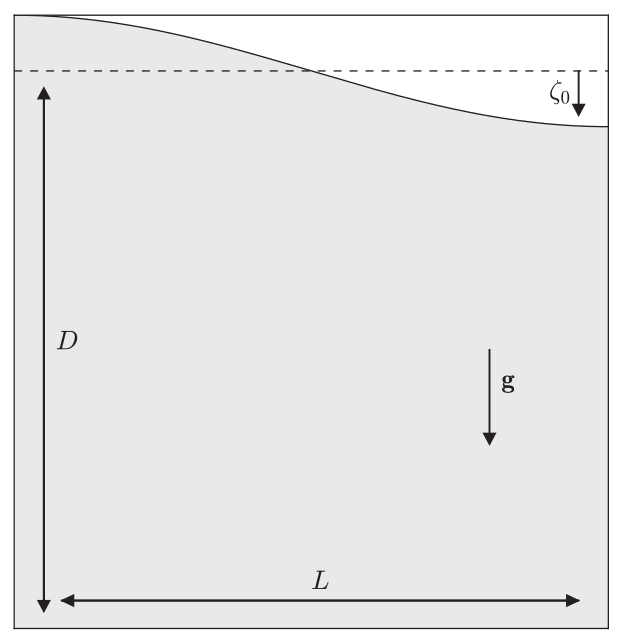
\includegraphics[height=0.8\textwidth]{images/benchmark_relaxation/robh17}\\
{\captionfont Taken from \cite{robh17}. Setup for the free surface relaxation benchmark.
For the tests $\rho=\eta=g=L=D=1$ and $\xi_0=0.005$.}
\end{minipage}\hfill
\begin{minipage}{0.45\textwidth}
\centering
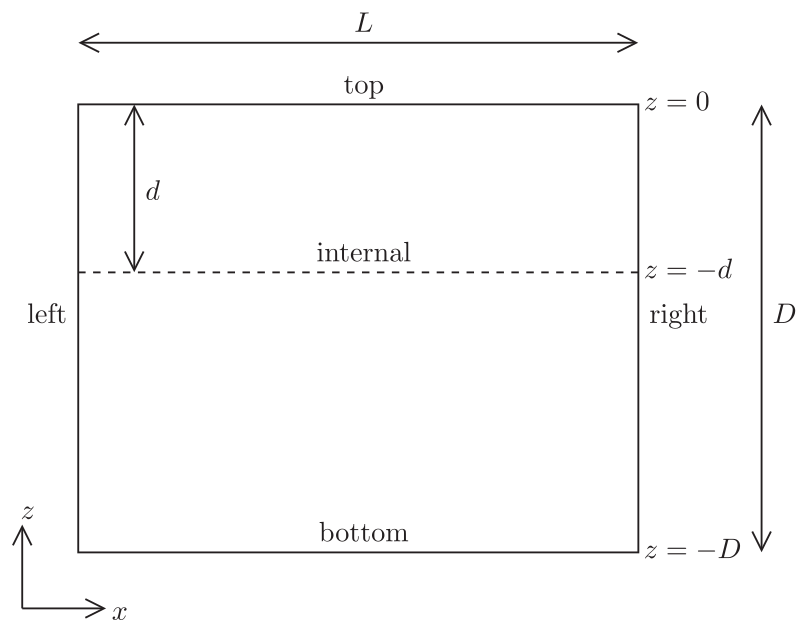
\includegraphics[height=0.8\textwidth]{images/benchmark_relaxation/krwd12}\\
{\captionfont Taken from \cite{krwd12}. $D=3\cdot 10^6$,$\eta=10^{21}$, $\rho=4500$, $g=10$, $\xi_0=10^3$m, and 
$L=D/4,D/2,D,2D,4D$.}
\end{minipage}
\end{center}
and the infinitesimal sinusoidal perturbations to the free surface is given by
\[
\xi(x,t=0)=\xi_0 \cos \left( \frac{2 \pi n x}{L}  \right)
\]
where $n$ is a wavenumber which is an integer multiple of 1/2 (taken to be 1/2 exactly in both cases).


%...............................................................
\subsubsection{the plastic brick}

\Literature \cite{hans03,moml07,lemm08,kaus10,egat10,qurj09,mishin11,maie12,spmw16,gltf18,frbt19,aspectmanual}

Pretty much all of the brick-type (elasto-)visco-plastic experiments in the literature
introduce a weak seed at the bottom of the domain to seed deformation (the shear bands
will ultimately stem from it). 
Dimensioned and dimensionless experiments have been carried out, with or without 
elastic behaviour, with or without adaptive mesh refinement, with first order and 
second order quadrilateral elements or Taylor-Hood triangles, with or without 
Newton algorithm, in extension and compression, with or without time-stepping,
with or without viscous lower layer. 


\begin{center}
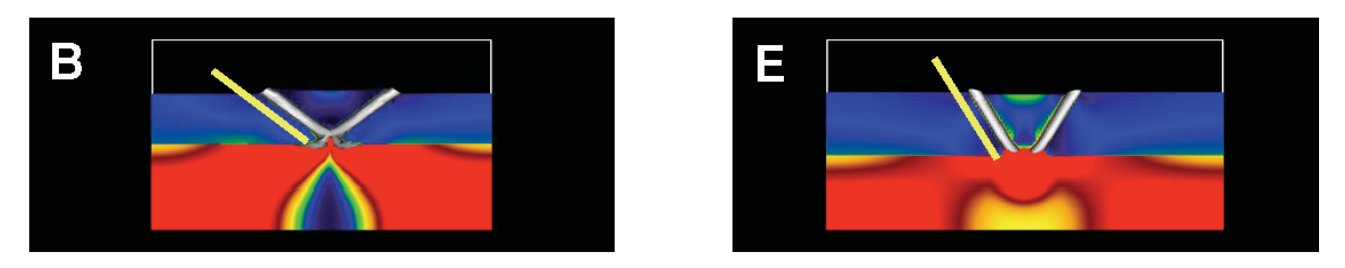
\includegraphics[width=7cm]{images/benchmark_brick/momu06}\\
{\captionfont Moresi \& M{\"u}lhaus, 2006 \cite{momu06}}
\end{center}

\begin{center}\noindent\rule{8cm}{0.4pt}\end{center}

\begin{center}
\begin{minipage}{0.45\textwidth}
\centering
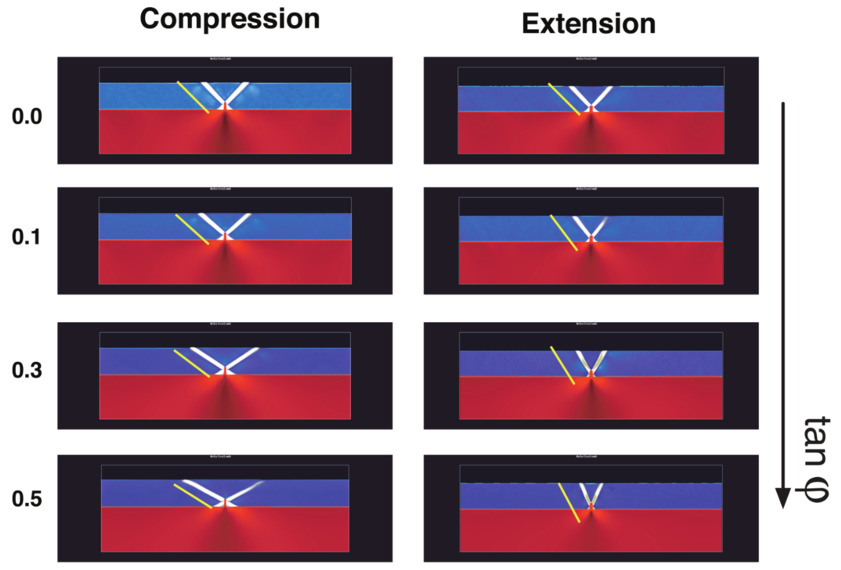
\includegraphics[height=0.8\textwidth]{images/benchmark_brick/moml07}\\
{\captionfont Moresi et al, 2007 \cite{moml07}}
\end{minipage}\hfill
\begin{minipage}{0.45\textwidth}
\centering
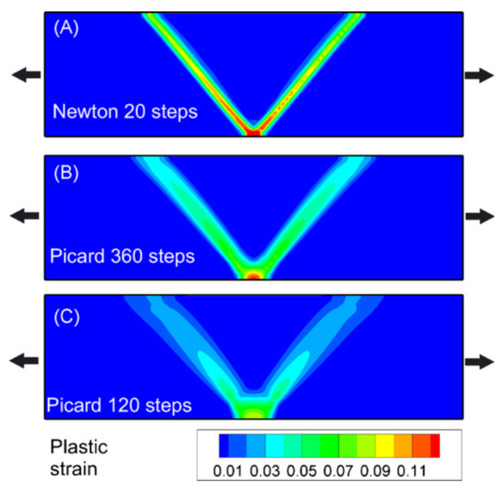
\includegraphics[height=0.8\textwidth]{images/benchmark_brick/poso08}\\
{\captionfont Popov et al, 2008 \cite{poso08}}
\end{minipage}
\end{center}

\begin{center}\noindent\rule{8cm}{0.4pt}\end{center}

\begin{center}
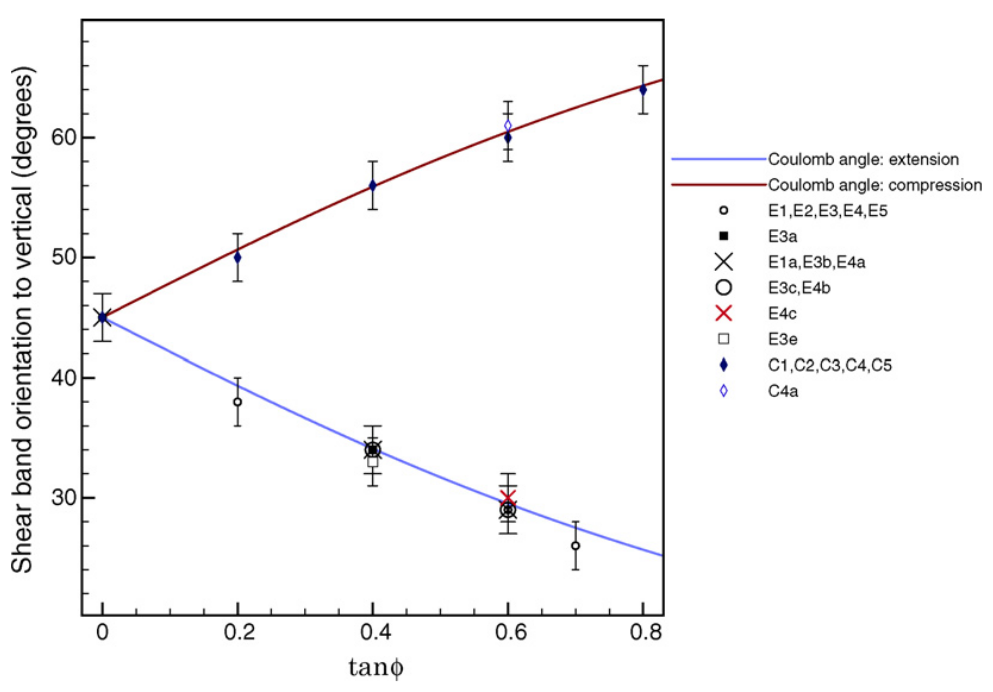
\includegraphics[width=5cm]{images/benchmark_brick/lemm08a}
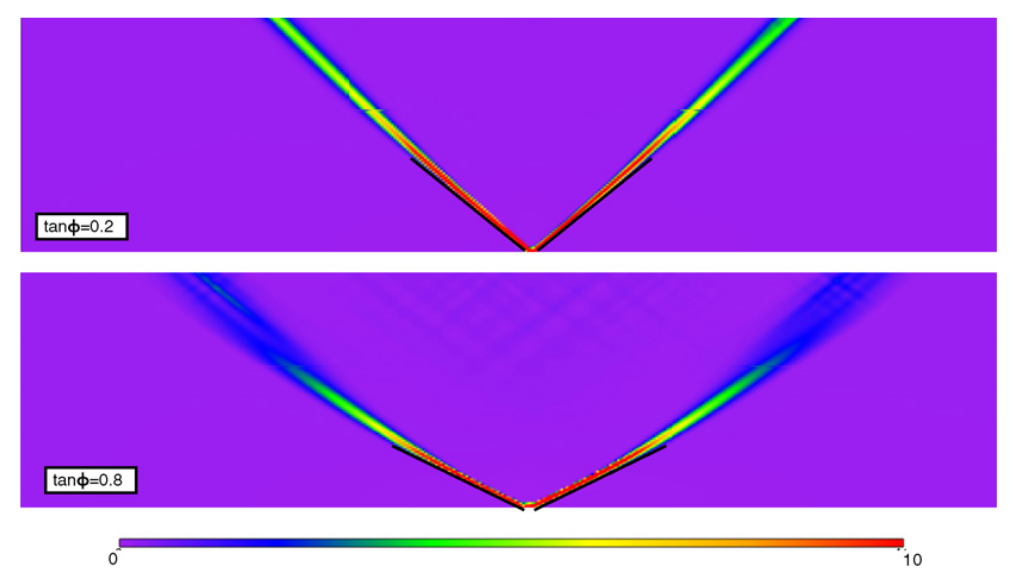
\includegraphics[width=5cm]{images/benchmark_brick/lemm08b}
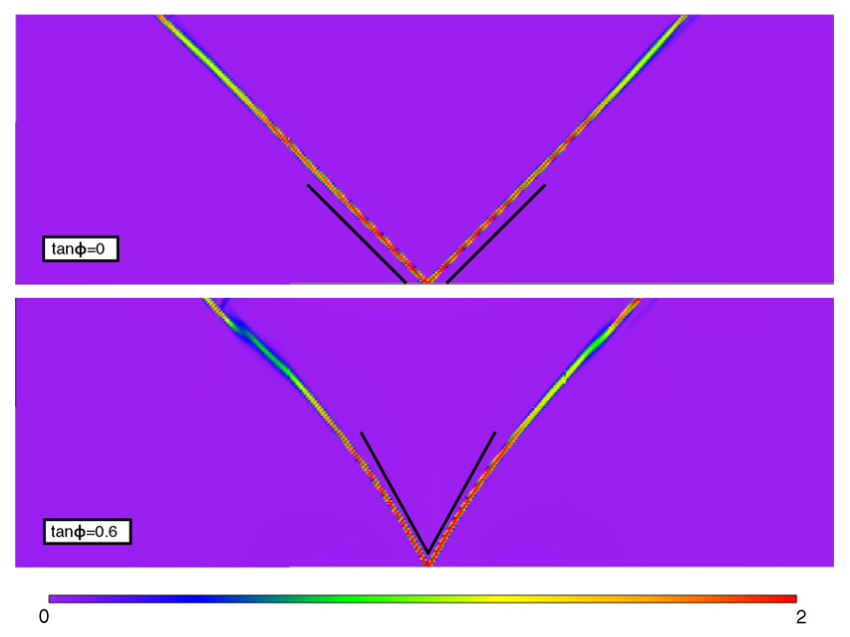
\includegraphics[width=5cm]{images/benchmark_brick/lemm08c}\\
{\captionfont Lemiale et al, 2008 \cite{lemm08}}
\end{center}

\begin{center}\noindent\rule{8cm}{0.4pt}\end{center}

\begin{center}
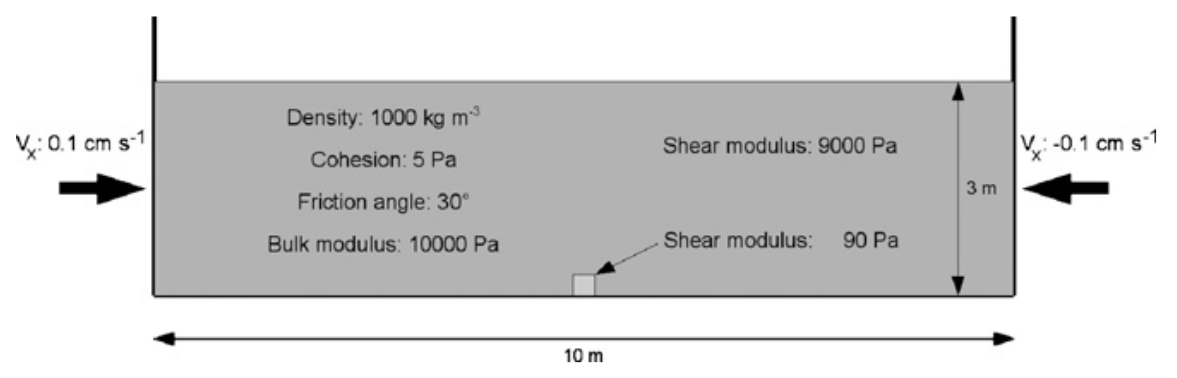
\includegraphics[width=7cm]{images/benchmark_brick/qurj09b}
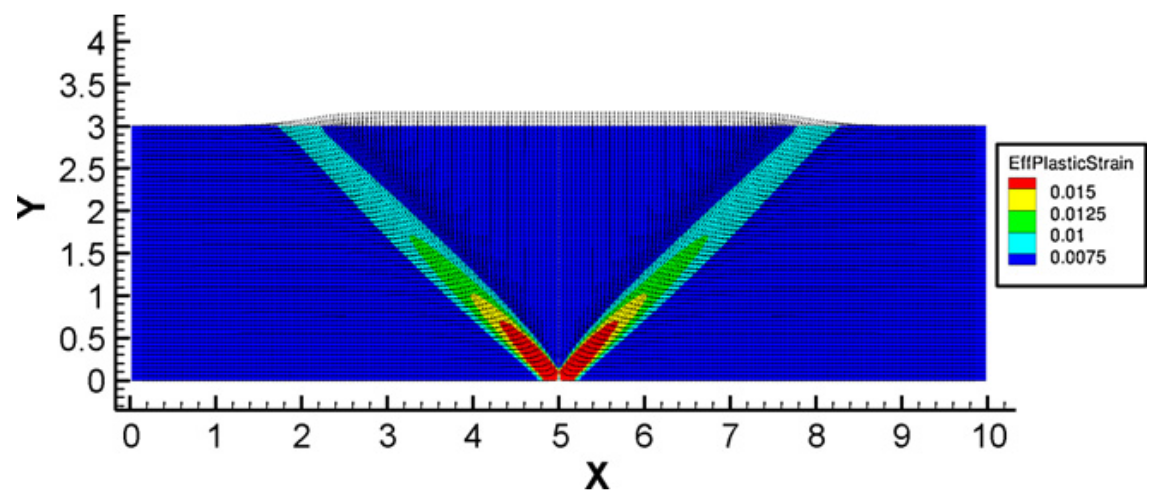
\includegraphics[width=6cm]{images/benchmark_brick/qurj09a}\\
{\captionfont Quinteros et al., 2009 \cite{qurj09}}
\end{center}

\begin{center}\noindent\rule{8cm}{0.4pt}\end{center}

\begin{center}
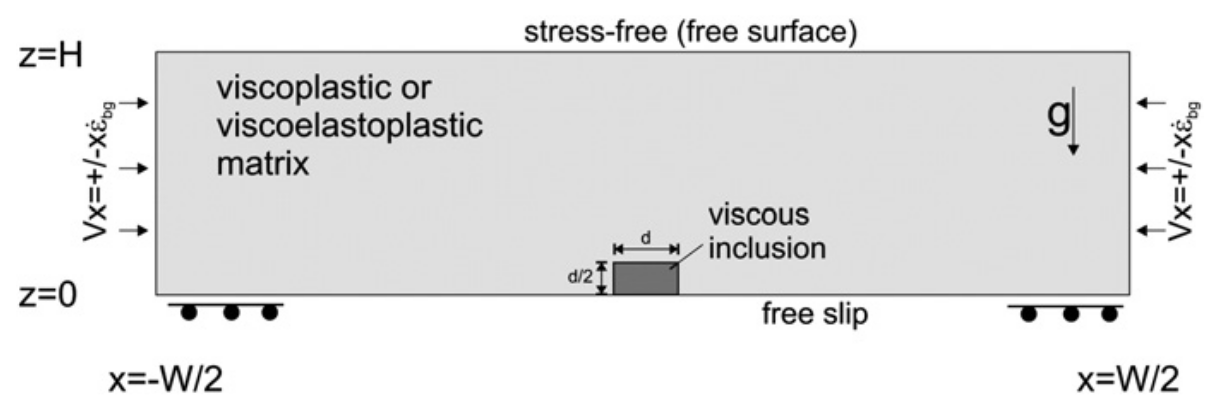
\includegraphics[width=5cm]{images/benchmark_brick/kaus10a}
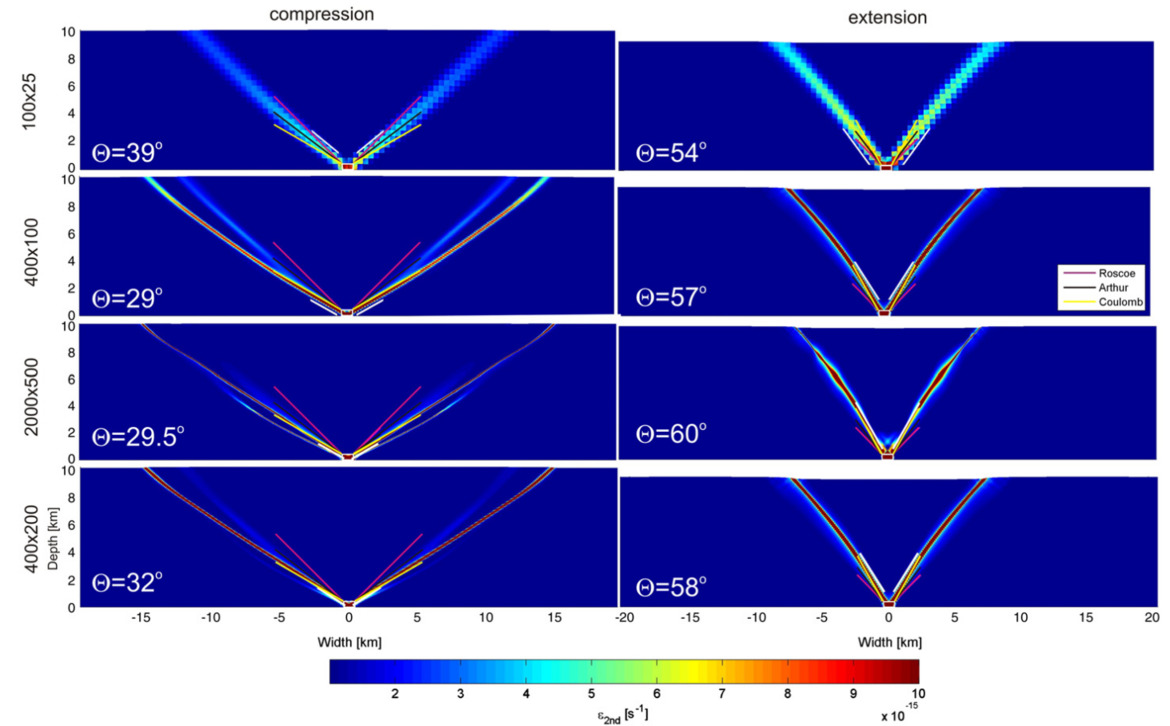
\includegraphics[width=5cm]{images/benchmark_brick/kaus10b}
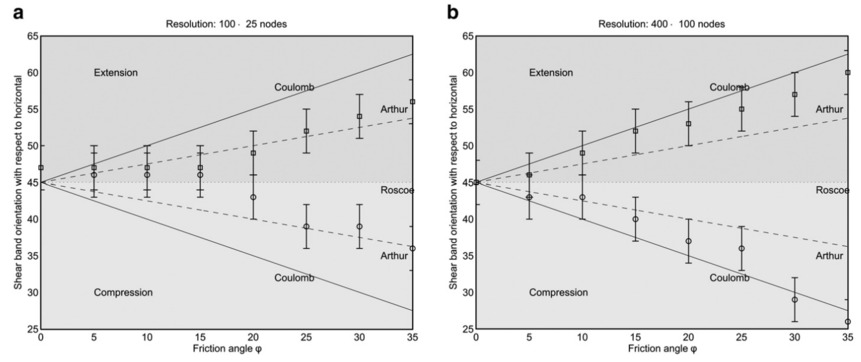
\includegraphics[width=5cm]{images/benchmark_brick/kaus10c}\\
{\captionfont Kaus, 2010 \cite{kaus10}}
\end{center}

\begin{center}\noindent\rule{8cm}{0.4pt}\end{center}

\begin{center}
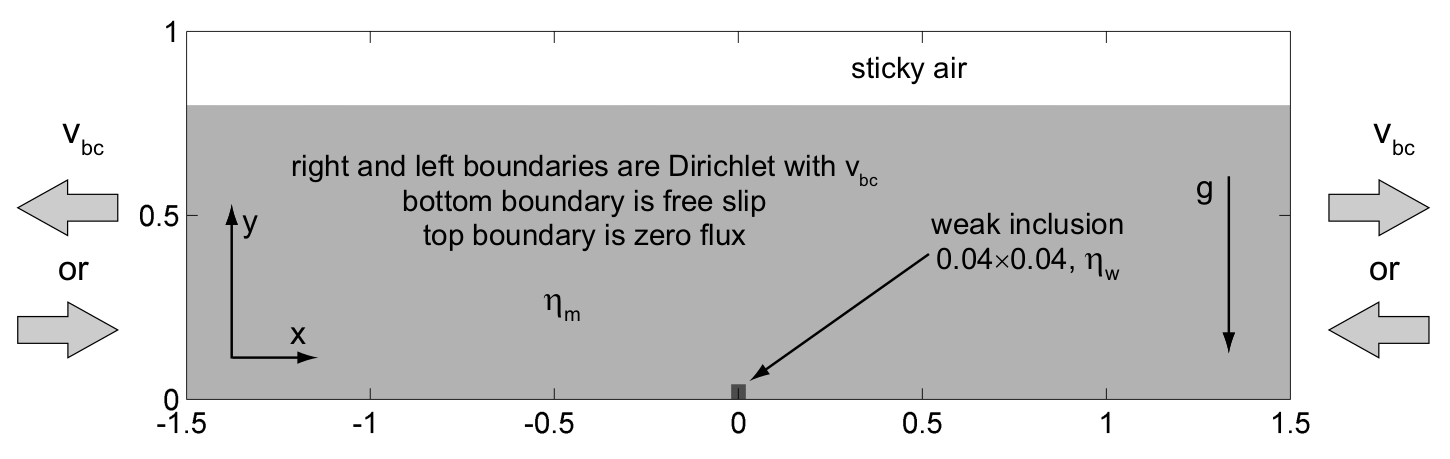
\includegraphics[width=3.74cm]{images/benchmark_brick/mishina}
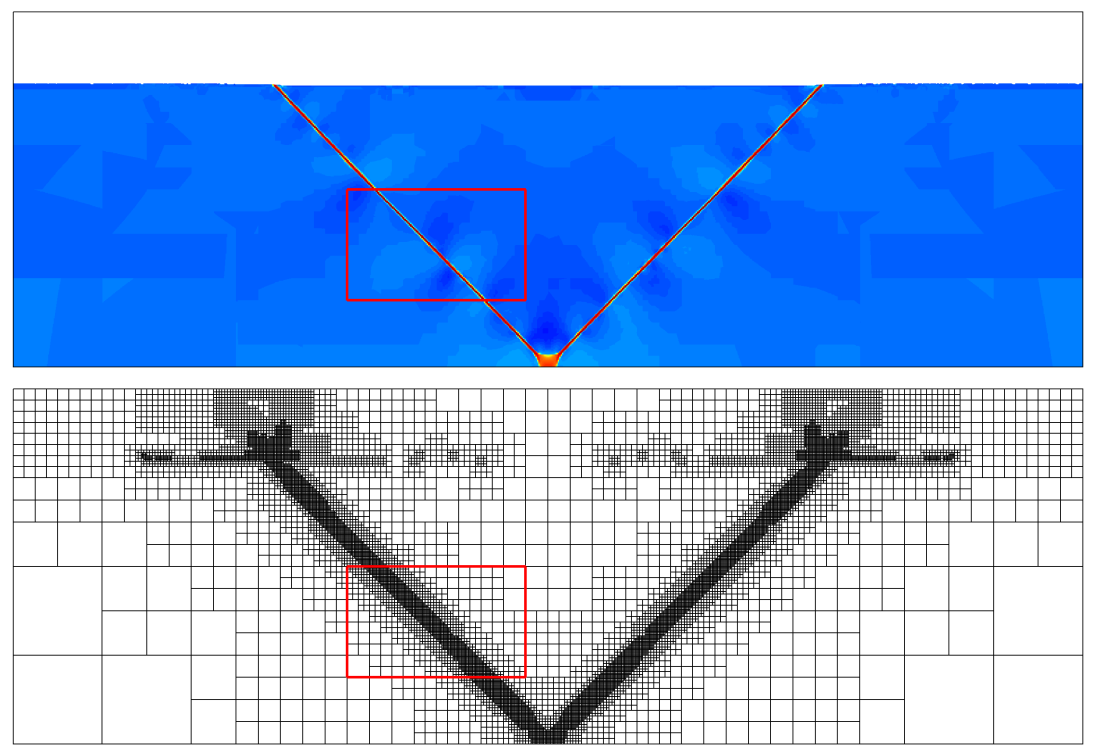
\includegraphics[width=3.74cm]{images/benchmark_brick/mishinb}
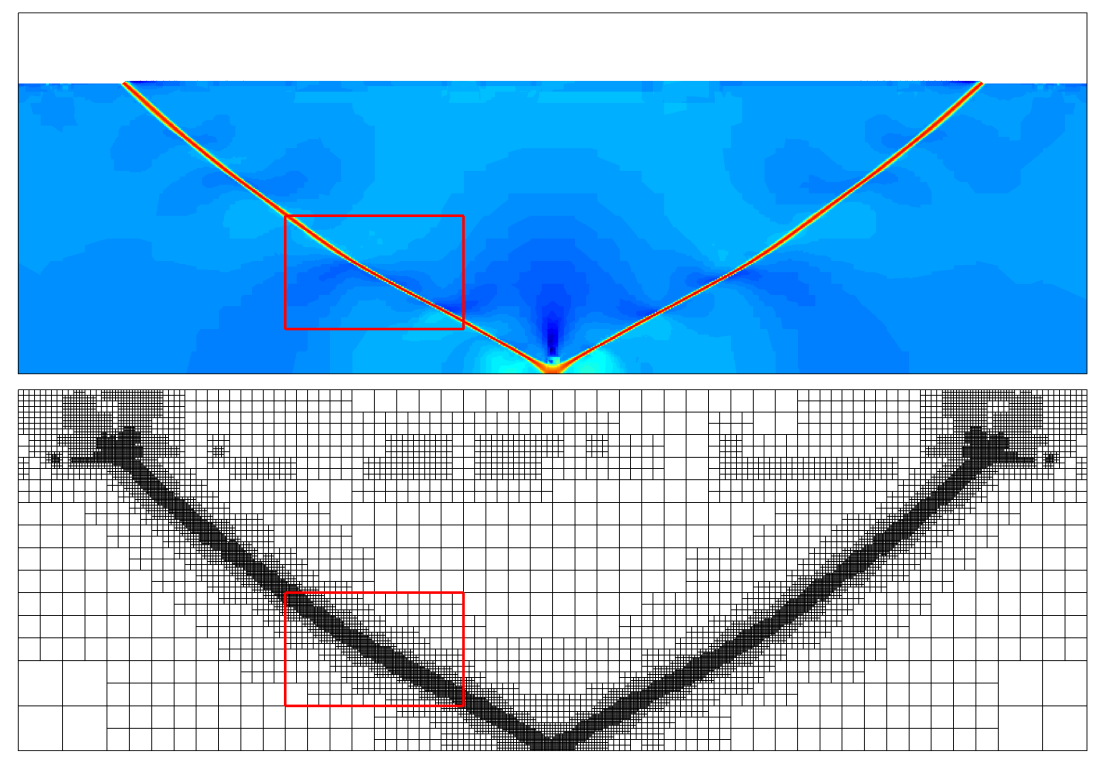
\includegraphics[width=3.74cm]{images/benchmark_brick/mishinc}
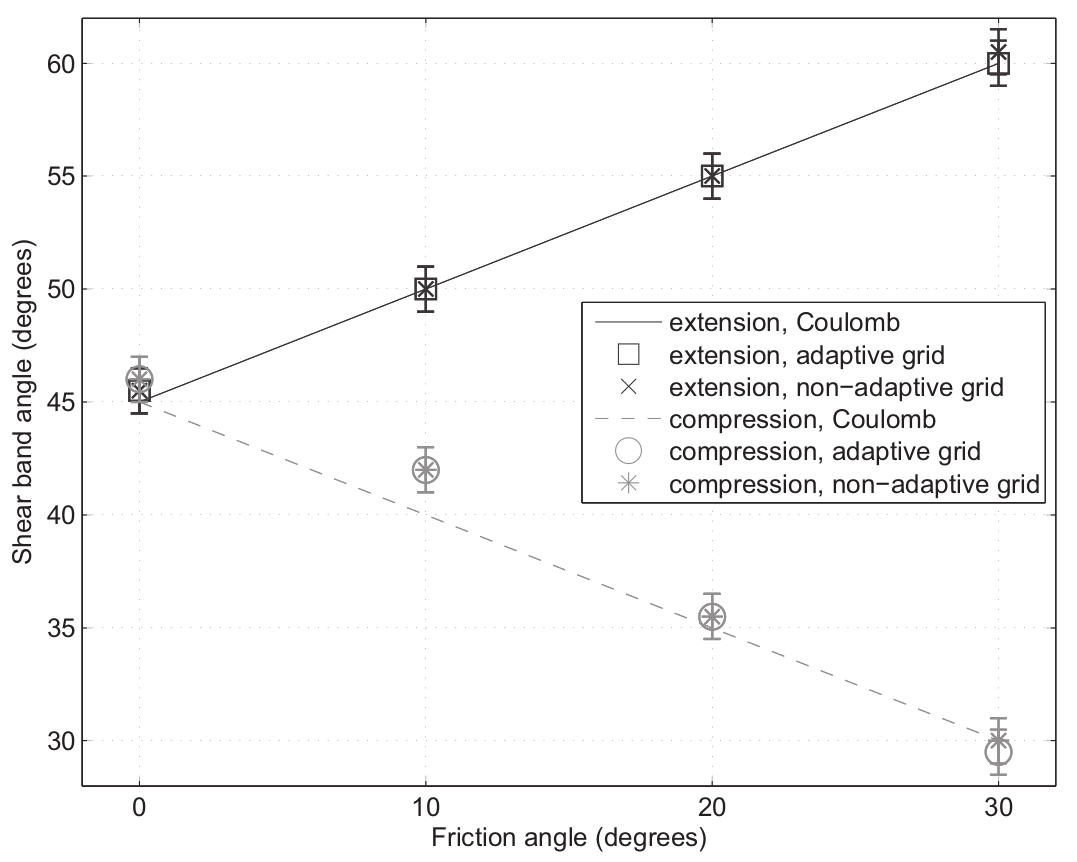
\includegraphics[width=3.74cm]{images/benchmark_brick/mishind}\\
{\captionfont Mishin, phd thesis, 2011 \cite{mishin11}}
\end{center}

\begin{center}\noindent\rule{8cm}{0.4pt}\end{center}

\begin{center}
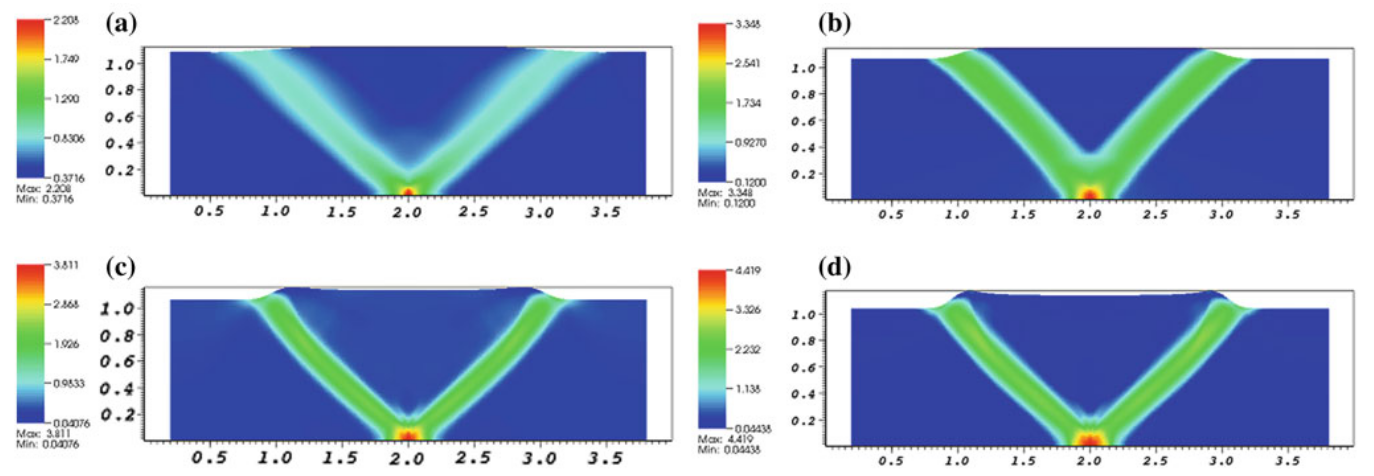
\includegraphics[width=9cm]{images/benchmark_brick/muso11}\\
{\captionfont M{\"u}hlhaus et al, 2011 \cite{muso11}.}
\end{center}

\begin{center}\noindent\rule{8cm}{0.4pt}\end{center}

\begin{center}
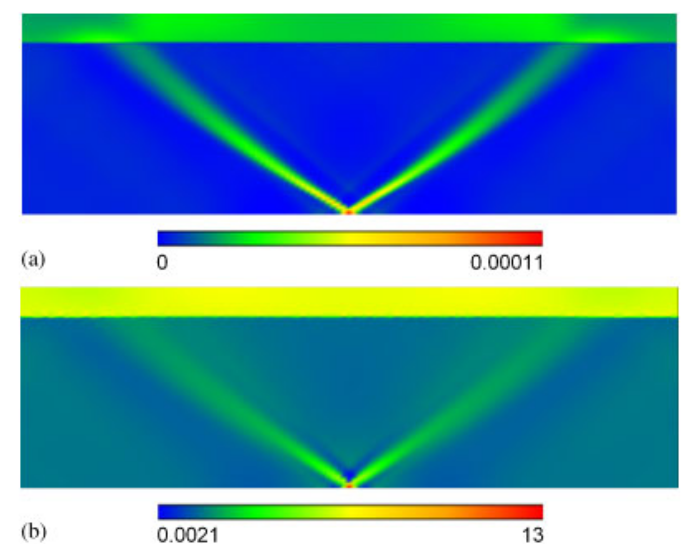
\includegraphics[width=9cm]{images/benchmark_brick/lemm11}\\
{\captionfont Lemiale et al, 2011 \cite{lemm11}.}
\end{center}

\begin{center}\noindent\rule{8cm}{0.4pt}\end{center}

\begin{center}
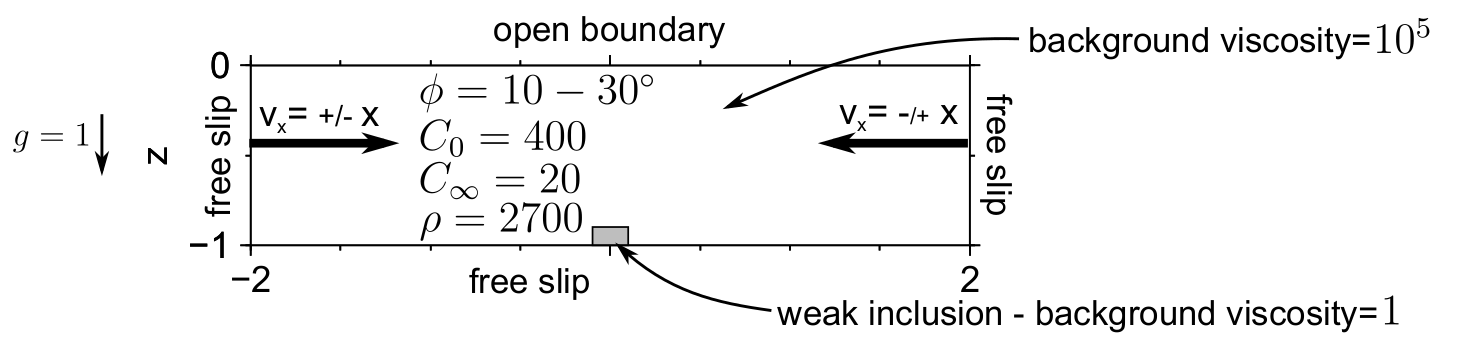
\includegraphics[width=8cm]{images/benchmark_brick/maie12a}
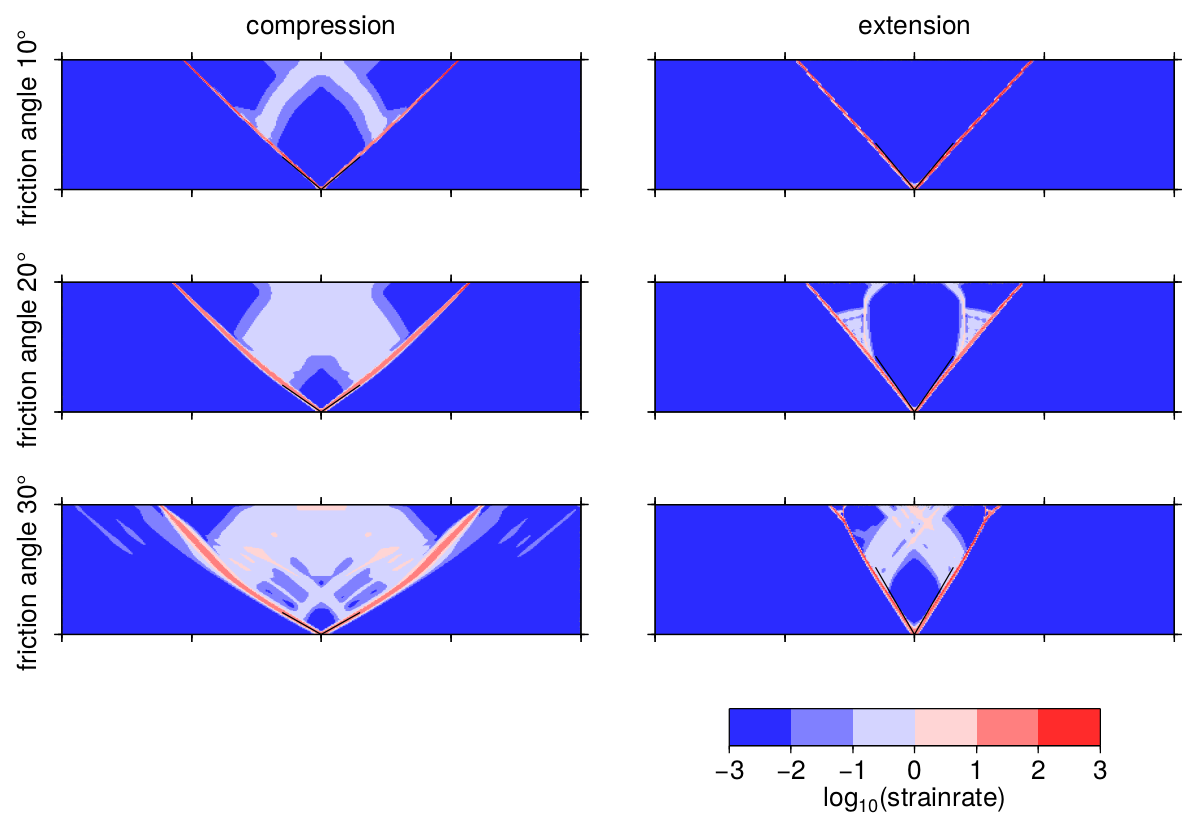
\includegraphics[width=5cm]{images/benchmark_brick/maie12b}\\
{\captionfont Maierova, phd thesis, 2012 \cite{maie12}}
\end{center}

\begin{center}\noindent\rule{8cm}{0.4pt}\end{center}

\begin{center}
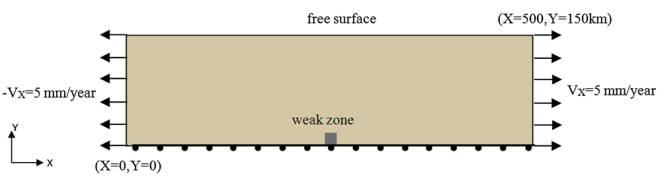
\includegraphics[width=5cm]{images/benchmark_brick/mofm13a}
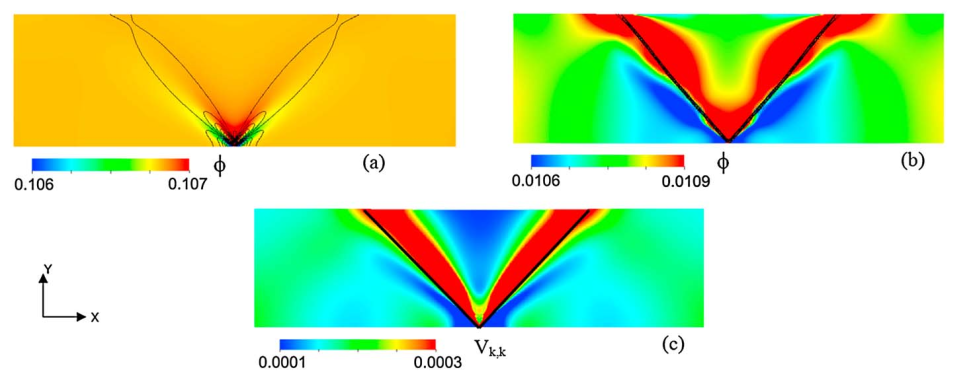
\includegraphics[width=8cm]{images/benchmark_brick/mofm13b}\\
{\captionfont Mohajeri et al, 2013 \cite{mofm13}.}
\end{center}

\begin{center}\noindent\rule{8cm}{0.4pt}\end{center}

\begin{center}
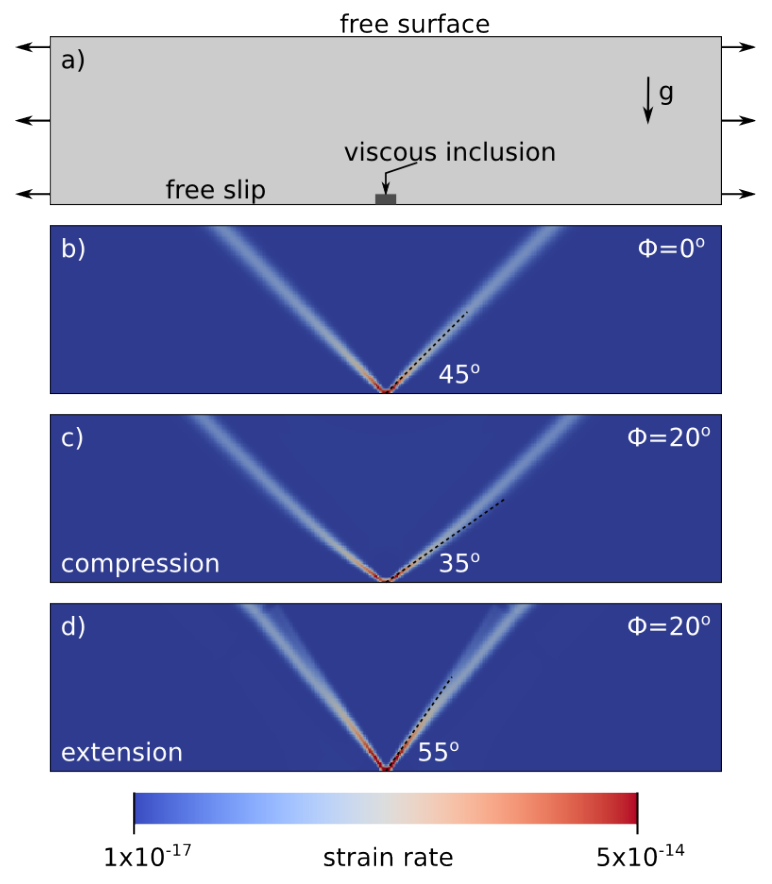
\includegraphics[width=5cm]{images/benchmark_brick/thie14a}
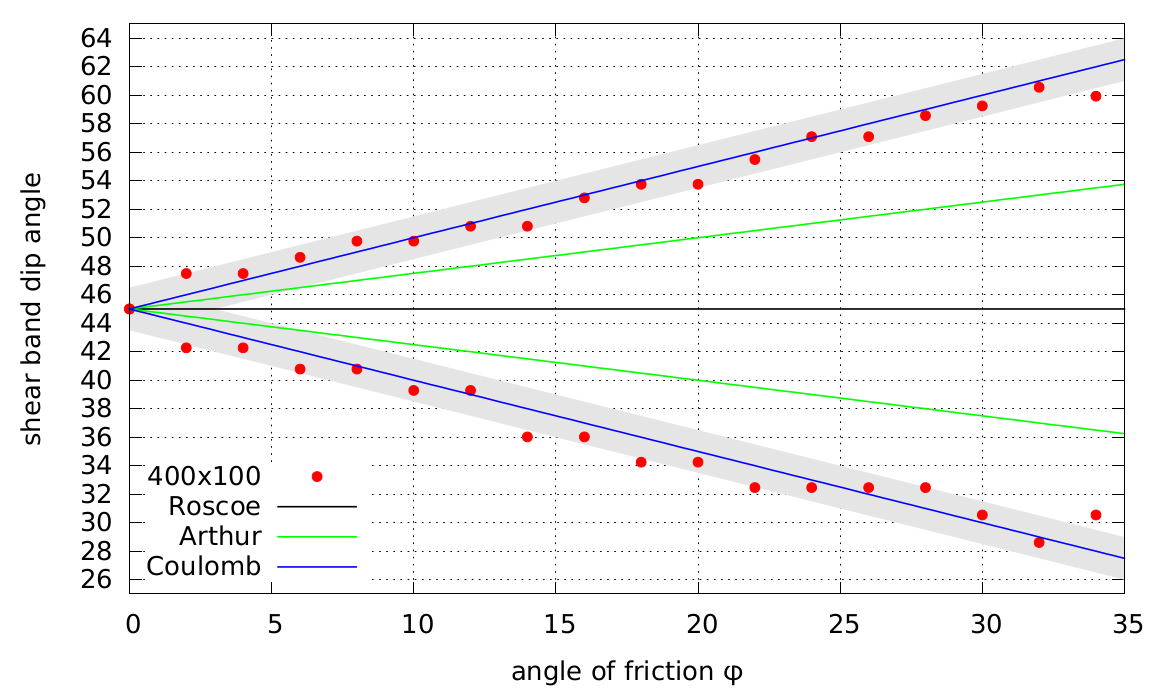
\includegraphics[width=8cm]{images/benchmark_brick/thie14b}\\
{\captionfont Thieulot, 2014 \cite{thie14}.}
\end{center}




\begin{center}\noindent\rule{8cm}{0.4pt}\end{center}

\begin{center}
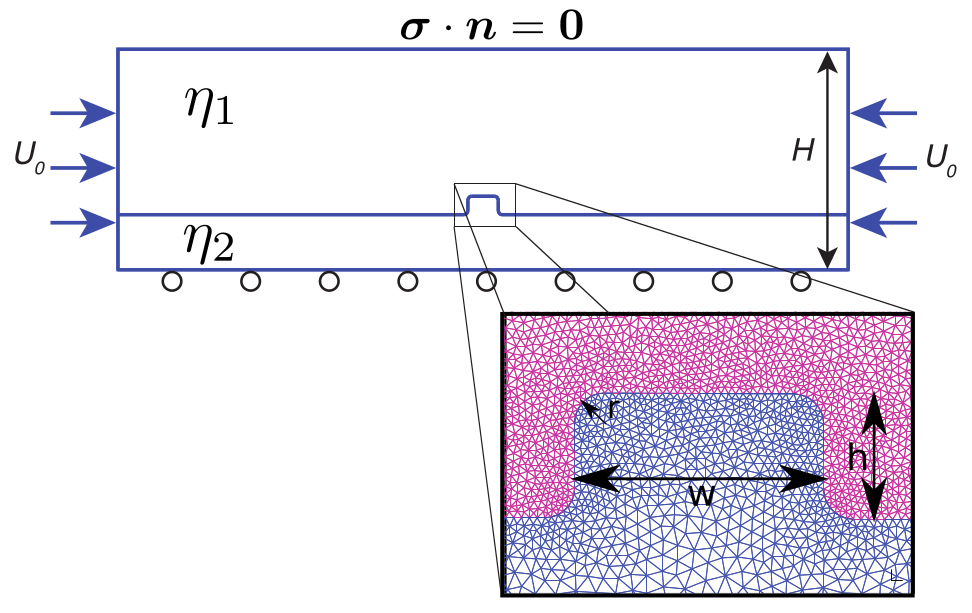
\includegraphics[width=5cm]{images/benchmark_brick/spmw16a}
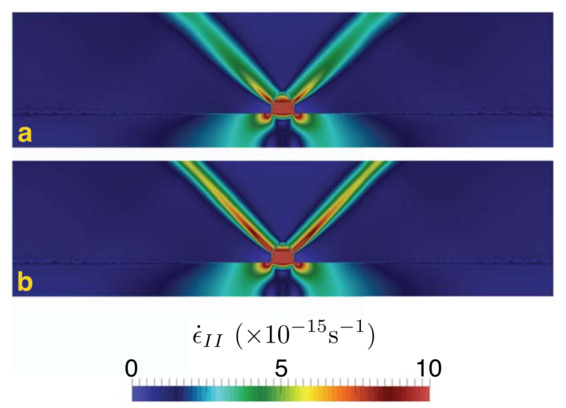
\includegraphics[width=5cm]{images/benchmark_brick/spmw16b}\\
{\captionfont Spiegelman et al, 2016 \cite{spmw16}}
\end{center}

\begin{center}\noindent\rule{8cm}{0.4pt}\end{center}

\begin{center}
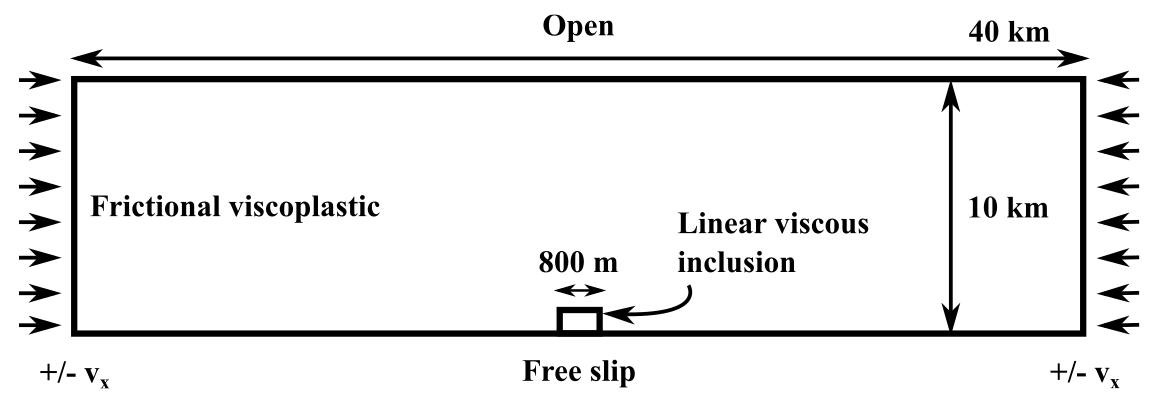
\includegraphics[width=5cm]{images/benchmark_brick/gltf18a}
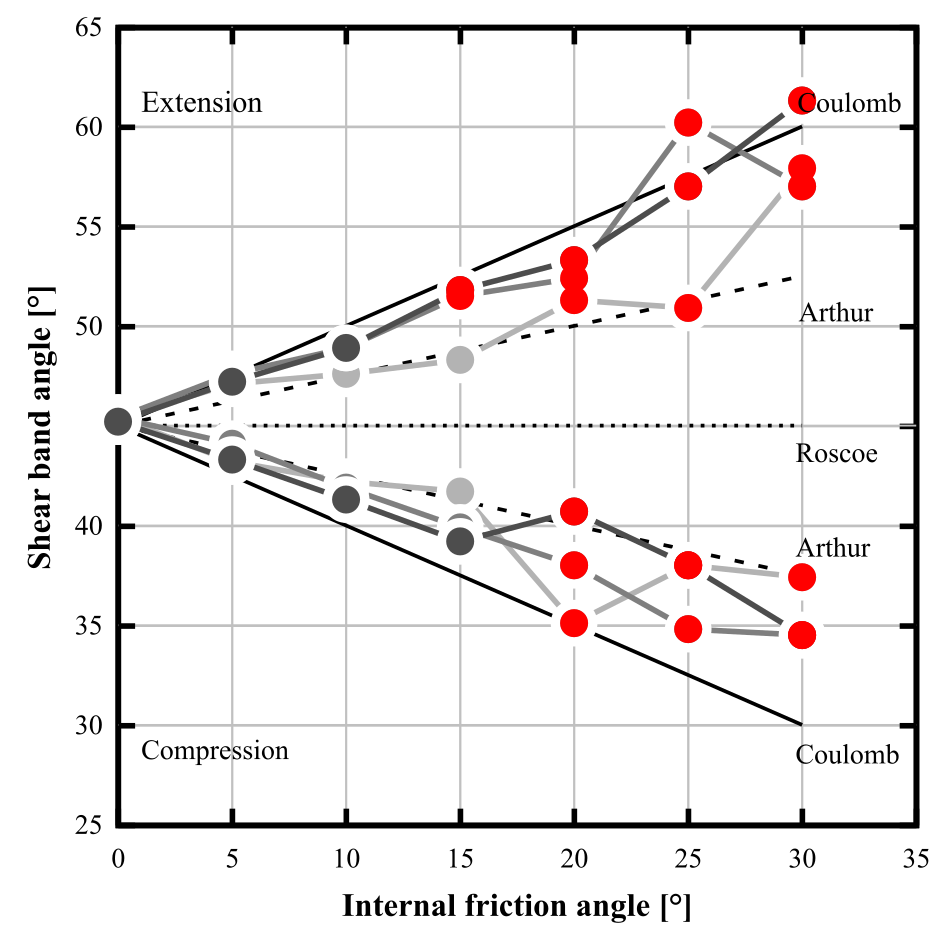
\includegraphics[width=5cm]{images/benchmark_brick/gltf18b}
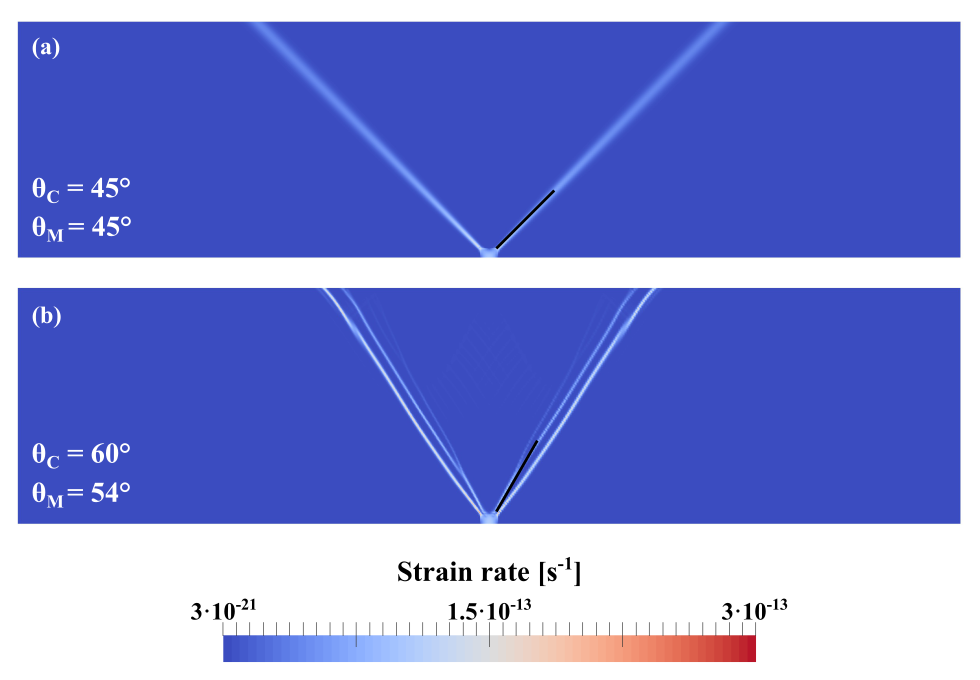
\includegraphics[width=5cm]{images/benchmark_brick/gltf18c}\\
{\captionfont Glerum et al, 2018 \cite{gltf18}}
\end{center}

\begin{center}\noindent\rule{8cm}{0.4pt}\end{center}

\begin{center}
\begin{minipage}{0.45\textwidth}
\centering
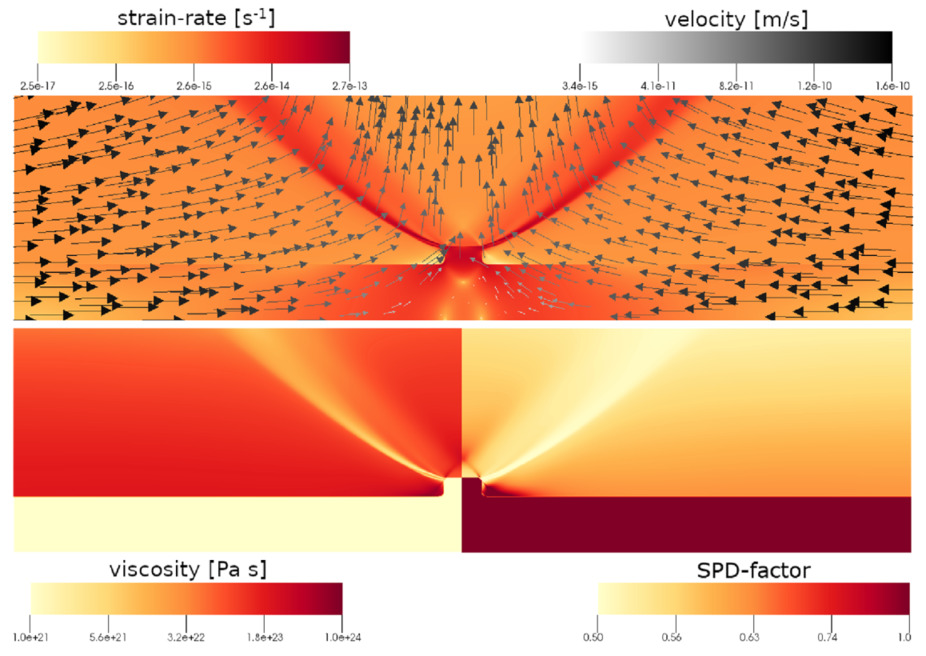
\includegraphics[height=0.8\textwidth]{images/benchmark_brick/frbt19}\\
{\captionfont Fraters et al, 2019 \cite{frbt19}}
\end{minipage}\hfill
\begin{minipage}{0.45\textwidth}
\centering
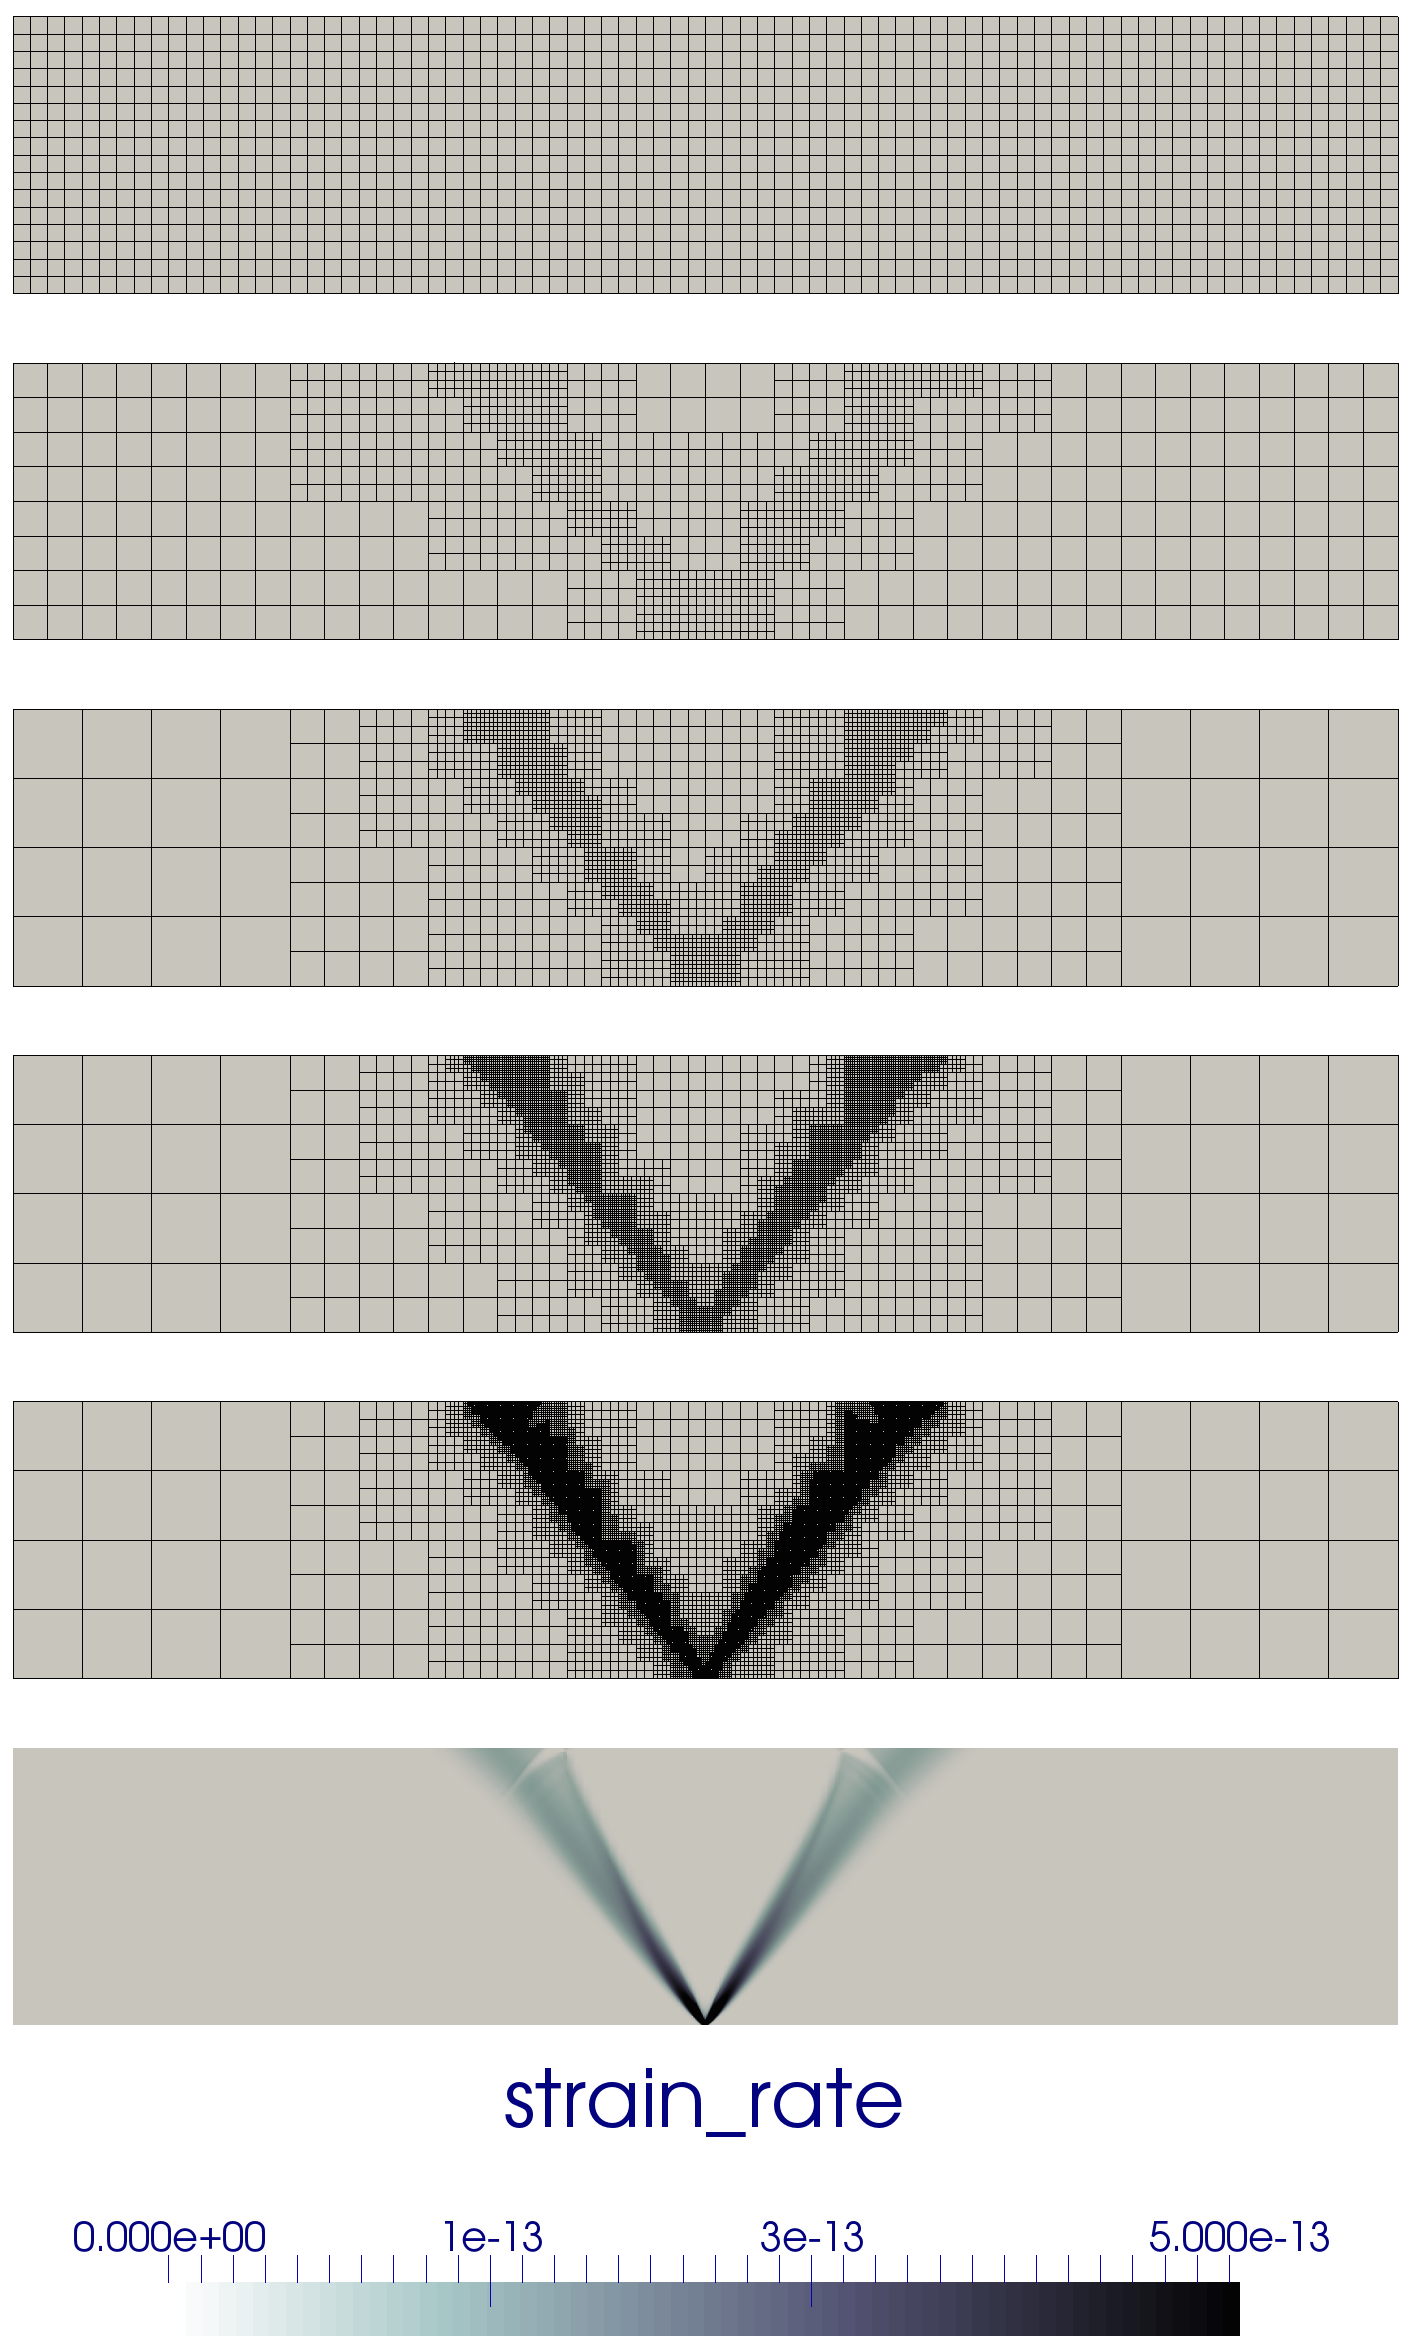
\includegraphics[height=0.8\textwidth]{images/benchmark_brick/aspectmanual}\\
{\captionfont Aspect manual \cite{aspectmanual}}
\end{minipage}
\end{center}

%..........................................................................
\subsubsection{Infinite plate with a circular hole \cite{rama16}}
\mscthesis \index{general}{MSc Thesis}

An infinite plate with a circular hole of radius $a$ 
is subjected to a unidirectional tensile load of $\sigma$ in the $x$ direction as shown
in the figure. In this case, only one quarter of the domain is analysed due
to symmetry along $x$ and $y$ axis. 

\begin{center}
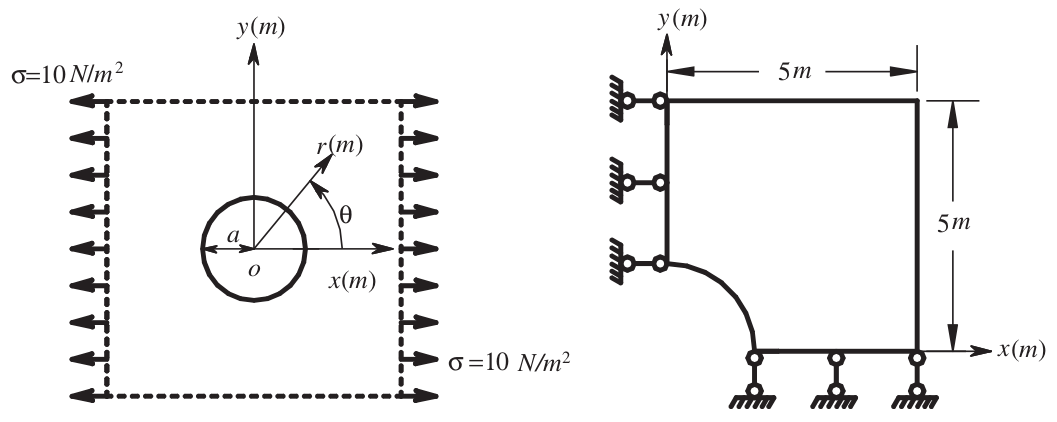
\includegraphics[width=0.65\textwidth]{images/benchmark_hole/yobu02}
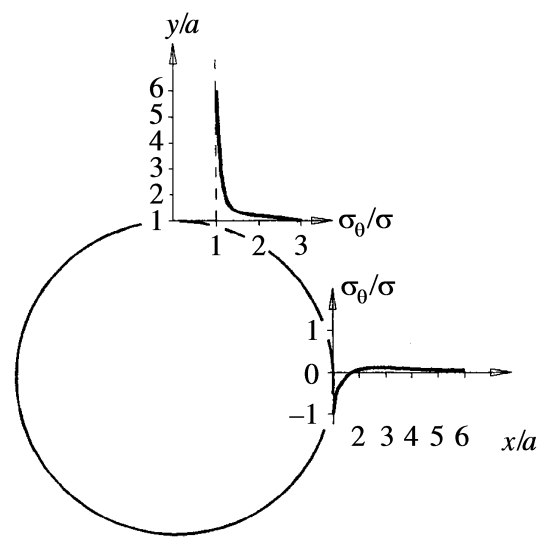
\includegraphics[width=0.25\textwidth]{images/benchmark_hole/yobu02b}\\
{\captionfont Left: An infinite plate with a circular hole subjected to unidirectional tension 
and its quarter model with symmetric conditions imposed on the left and bottom edges.
Right: Tangential stress distribution for $\theta=0$  and $\theta=\pi/2$. \cite{yobu02}}
\end{center}

The inner boundary of the hole is traction free and the right edge was
imposed with the tractions based on the analytical solutions.
The left edge is constrained in the $x$ direction and the bottom
edge is constrained in the $y$ direction, respectively. The plane stress
condition is considered and the parameters are: 
Young modulus $E=$3e7 MPa, Poisson Ratio $\nu=$0.3, Load $\sigma$=10 N/m$^2$, a=1m.

The analytical stress components for this
problem are 

\begin{eqnarray}
\sigma_{xx}(x,y) &=& \sigma \left(  1-\frac{a^2}{r^2}\left(\frac{3}{2}\cos 2\theta + \cos 4\theta \right) 
+ \frac{3a^4}{2r^4} \cos 4\theta \right) \\
\sigma_{yy}(x,y) &=& -\sigma \left( \frac{a^2}{r^2} \left(\frac{1}{2}\cos 2\theta - \cos 4\theta \right) 
- \frac{3a^4}{2r^4} \cos 4\theta \right) \\
\sigma_{xy}(x,y) &=& -\sigma \left( \frac{a^2}{r^2} \left(\frac{1}{2}\sin 2\theta + \sin 4\theta\right) 
+ \frac{3a^4}{2r^4} \sin 4\theta \right) 
\end{eqnarray}

Note that \cite{rama16} cites \cite{chnn10} which cites the book \cite[p772]{yobu02} 
which cites \cite{budynas} for the solution!
\todo[inline]{there are discrepancies between \cite{rama16} and \cite{chnn10}}

Following \cite{yobu02}, it can be shown, from linear elasticity, that the tangential
stress throughout the plate is given by
\[
\sigma_\theta = \frac{\sigma}{2} \left[ 1+\frac{a^2}{r^2} - \left( 1+3\frac{a^4}{r^4}  \right) \cos 2\theta   \right]
\]
The maximum stress is $\sigma_\theta=3\sigma$ at $r=a$ and $\theta=\pm \pi/2$. Along the surface of the hole, 
the tangential stress is $-\sigma$ at y $\theta=0$  and $\theta=\pi$, 
and increases, as $\theta$ increases, to $3\sigma$ at $\theta=\pi/2$ and $\theta=3\pi/2$.
 

%..............................................................................
\subsubsection{Slope stability for elasto-plastic materials a la \cite{rama16}}
\mscthesis \index{general}{MSc Thesis}

The bottom of the domain is constrained and the model is 
subjected to gravitational load. The material properties considered are

Young modulus 20e3 MPa, Poisson Ratio 0.49, Constitutive law Mohr-Coulomb 
(friction angle $\phi=20$\degree, 
dilatancy angle $\phi=20$\degree, cohesion $c$=50Mpa).

\begin{center}
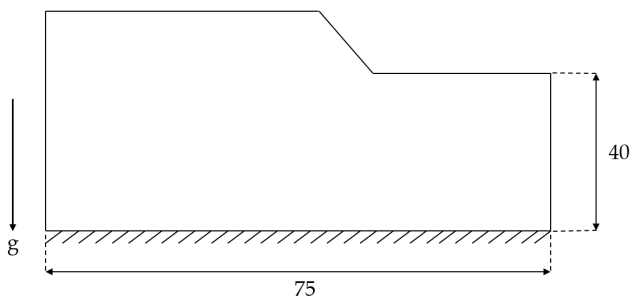
\includegraphics[width=0.5\textwidth]{images/benchmark_slope/rama16c}
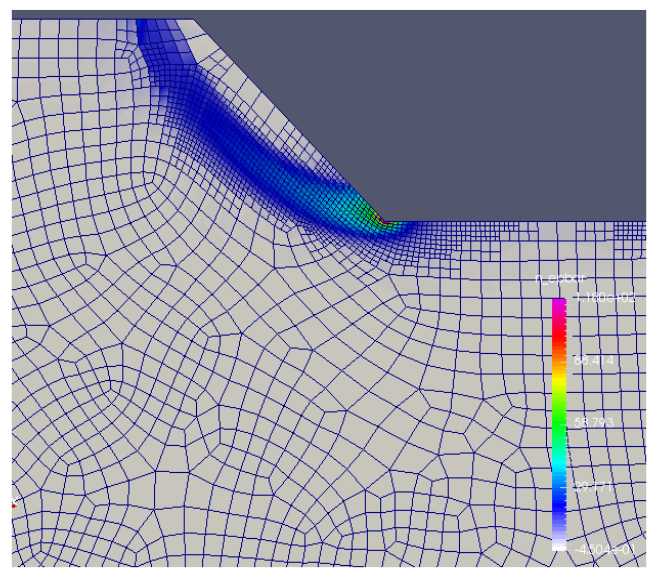
\includegraphics[width=0.4\textwidth]{images/benchmark_slope/rama16b}\\
{\captionfont Left: Slope stability problem setup; Right: Adaptive Refinement based 
on Plasticity Indicator}
\end{center}


%..............................................................................
\subsubsection{Time-dependent benchmark in an annulus}\label{sec:tdba}

This benchmark is presented in Gass{m\"o}ller et al \cite{galb19}.
The domain is a 2D annulus with inner and outer radii $R_1=1$ and $R_2=2$, respectively.
In this situation, the incompressible isothermal Stokes equations and their solution
can be expressed in a cylindrical coordinate system in terms of the radius $r$ and the
azimuthal angle $\theta$. The viscosity is set to $eta=1$, and the density is given by
\begin{equation}
\rho(r,\theta)=48r^5
\end{equation}
The gravity vector is set to 
\begin{equation}
\vec{g}(r,\theta)=\frac{r^3}{384} \vec{e}_r + \vec{e}_\theta
\end{equation}
Note that this gravity vector is not the gradient of a gravity potential
and consequently not physical.
The Stokes system can then be solved using a separation of variables
approach and yields
\begin{equation}
\vec{\upnu}=-r^7 \vec{e}_\theta
\quad\quad
p(r,\theta)=\frac{r^9}{72}-\frac{512}{72}
\end{equation}
\begin{center}
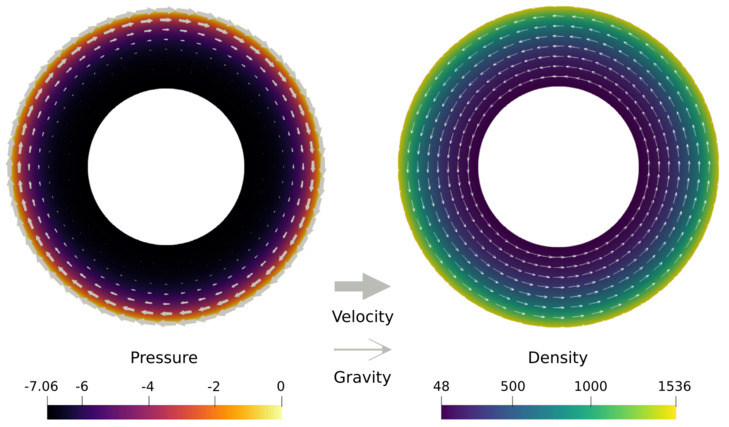
\includegraphics[width=12cm]{images/benchmark_annulus/galb19}\\
{\captionfont Taken from \cite{galb19}}
\end{center}
Rather importantly, this benchmark was arrived at by means of a stream function (see Section~\ref{sec:streamfunction}) 
$\psi(r,\theta)=F(r)G(\theta)$ with $F(r)=r^8/8$ and $G(\theta)=1$.

%..............................................................................
\subsubsection{Convection in 2D-box} \label{sec:citb}

We start from the following stream function (see Section~\ref{sec:streamfunction}):
\begin{equation}
\psi(x,y)=\frac{1}{\pi} \sin \pi x \sin \pi y
\end{equation}
which yields:
\begin{eqnarray}
u(x,y)&=&\frac{\partial \psi}{\partial y} = \sin \pi x \cos \pi y \nn\\
v(x,y)&=&-\frac{\partial \psi}{\partial x} = - \cos \pi x \sin \pi y
\end{eqnarray}
The pressure field is 
\begin{equation}
p(x,y) = 2\pi \cos (\pi x) \cos (\pi y) 
\end{equation}
with 
\begin{equation}
\rho(x,y)=\sin(\pi x) \sin (\pi y)
\qquad\qquad
g_y = -4\pi ^2 \frac{\cos (\pi x)}{\sin (\pi x)}
\end{equation}

\begin{center}
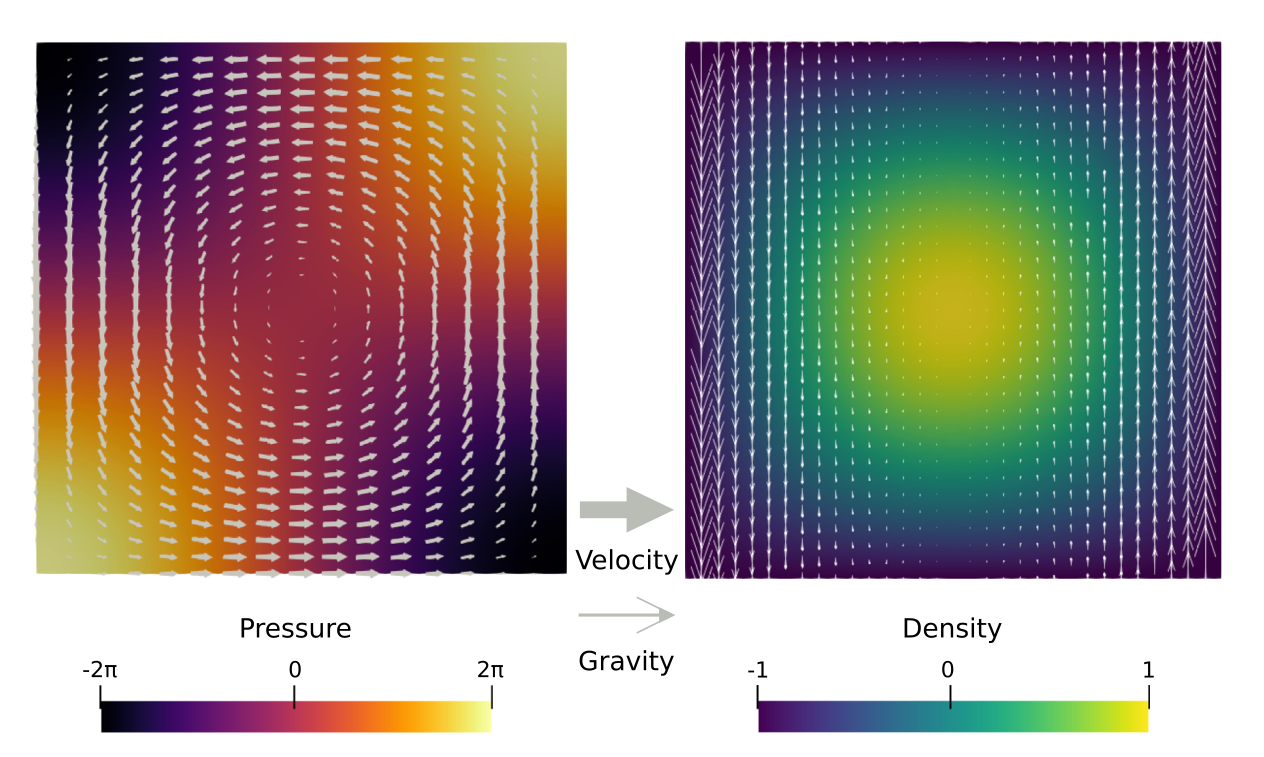
\includegraphics[width=12cm]{images/benchmark_convbox/galb19}\\
{\captionfont Taken from \cite{galb19}}
\end{center}

\begin{eqnarray}
v_{rms} 
&=& \sqrt{\frac{1}{L_xL_y} \int_0^1 \int_0^1 (u^2+v^2) dxdy} \nn\\
&=& \sqrt{\int_0^1 \int_0^1 ( \sin^2 (\pi x) \cos^2 (\pi y) + \cos^2 (\pi x) \sin^2 (\pi y) ) dxdy} \nn\\
&=& \sqrt{ \int_0^1 \sin^2 (\pi x) dx  \cdot \int_0^1 \cos^2 (\pi y) dy + \int_0^1 \cos^2 (\pi x) dx \cdot \int \sin^2 (\pi y) dy } \nn\\
&=& \sqrt{\frac{1}{2} \frac{1}{2}+ \frac{1}{2} \frac{1}{2} }\nn\\
&=& \frac{\sqrt{2}}{2} \nn\\
&\simeq& 0.70711...
\end{eqnarray}


%..............................................................................
\subsubsection{The sinker problem}\label{sec:sinker}

This experiment is not a benchmark stricto sensu since there is no analytical solution. However, it is widely used in the technical literature because of its simple setup and since it allows to test solving strategies.
Also, it can conveniently be carried out in both two and three dimensions.

\paragraph{In two dimensions} The time dependent version of the experiment is for instance to be found 
in Gerya \cite{gery10} and the same is repeated in Thieulot \cite{thie11}.

This simple benchmark provides challenging numerical experiments 
dealing with large viscosity variations within the simulation
domain. It consists of a bulk of fluid 1 ($\eta_1,\rho_1$) 
in which a block of fluid 2 ($\eta_2,\rho_2$) falls under its own
weight. The domain is a square of size $L_x = L_y = 500$ km and the
block is initially centred at point ($x$ = 250 km, $y$ = 400 km) with size
$100 \times 100$ km.
Free slip boundary conditions are imposed on all sides of the domain. 
In \cite{thie11} five experiments have been conducted:
$\eta_1 = 10^{20}$ Pa.s, $\rho_2$ = 3220 kg/m$^3$ ;
$\eta_1 = 10^{21}$ Pa.s, $\rho_2$ = 3300 kg/m$^3$ ;
$\eta_1 = 10^{22}$ Pa.s, $\rho_2$ = 6600 kg/m$^3$ ;
$\eta_1 = 10^{23}$ Pa.s, $\rho_2$ = 3300 kg/m$^3$ ;
$\eta_1 = 10^{24}$ Pa.s, $\rho_2$ = 9900 kg/m$^3$,
while in all experiments the density of the surrounding fluid is
$\rho_1=3200$ kg/m$^3$ and the viscosity of the block is varied between
$10^{19}$ and $5\cdot10^{27}$ Pa.s.

\begin{center}
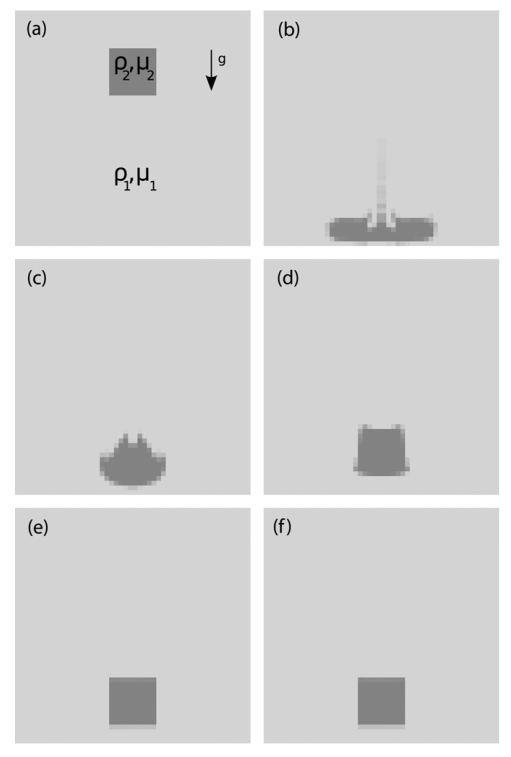
\includegraphics[width=5cm]{images/benchmark_sinker/thie11a}
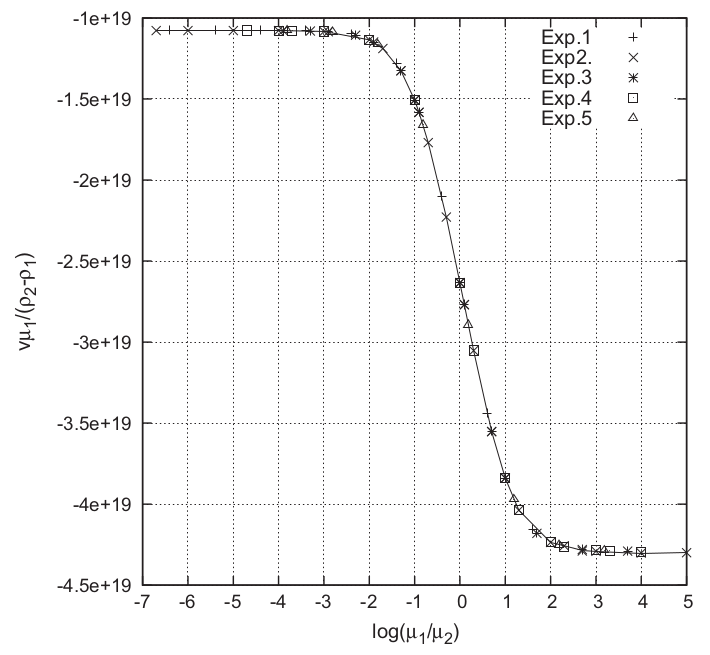
\includegraphics[width=7cm]{images/benchmark_sinker/thie11b}\\
{\captionfont Left: 
$\eta_1 = 10^{21}$ Pa.s, $\rho_2= 3300$ kg/m$^3$. 
(a) Initial setup; 
(b) $\eta_1 = 10^{21}$ Pa.s at time $t$ = 10 Myrs; 
(c) $\eta_1 = 10^{22}$ Pa.s at time $t$ = 20 Myrs; 
(d) $\eta_1 = 10^{23}$ Pa.s at time $t$ = 20 Myrs; 
(e) $\eta_1 = 10^{25}$ Pa.s at time $t$ = 20 Myrs; 
(f) $\eta_1 = 10^{27}$ Pa.s at time $t$ = 20 Myrs. 
Right: Velocity measurements as a function of the viscosity contrast between
surrounding medium and block for all experiments.
Taken from \cite{thie11}}
\end{center}

\paragraph{In three dimensions}
Let us look at the sinker experiment from Furuichi et al \cite{fumt11}: 
The domain is the unit box the origin at the center of the box. A cube with a viscosity $\eta_1=\Delta \eta$ 
and density $\rho_1 = 1$ was placed at the middle of the domain defined by
$-0.15 \leq x,y,z \leq 0.15$.
The material surrounding the cube has the properties $\eta_0=1$ and $\rho_0 = 0$. 
The body force of the momentum equation was taken as $(0, 0,-\rho g)$ with $g = 1$.
Along all walls on the domain, free-slip boundary conditions were employed.

\begin{center}
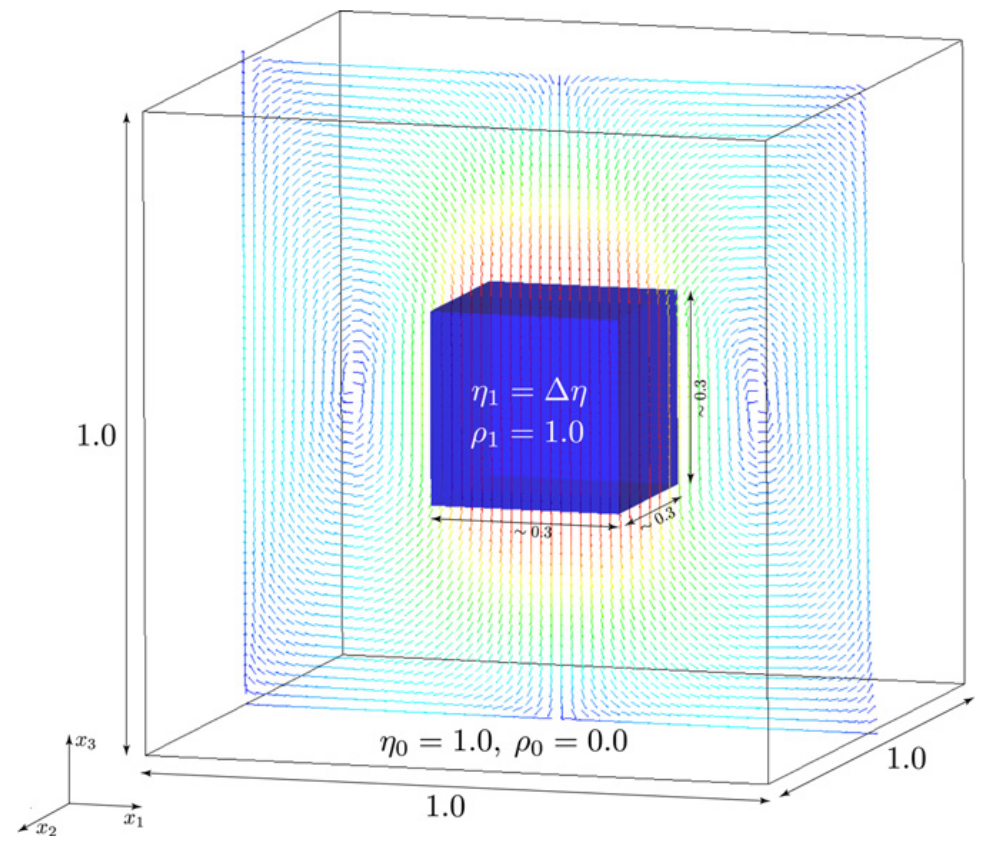
\includegraphics[width=8cm]{images/benchmark_sinker/fumt11}\\
{\captionfont Simulation setup for the 3D falling block (SINKER) problem. The vectors represent computed flow.
Taken from \cite{fumt11}}
\end{center}



%......................................................
\subsubsection{The hot blob problem}\label{sec:hotblob}

This is a very similar setup as the 3D sinker from the same authors
with higher but more diffusive variation of viscosity.
The body force is given by $(0, 0, \beta T)$ and
where the temperature field $T$ is defined by $T = \exp  (-\gamma (x^2+y^2+(z-0.3)^2))$ 
with the constant parameters $\beta=10^6$ and $\gamma=200$. 
The temperature-dependent viscosity $\eta = \exp( -\alpha T)$ is employed with the parameter for viscosity
contrast $\alpha$.

\begin{center}
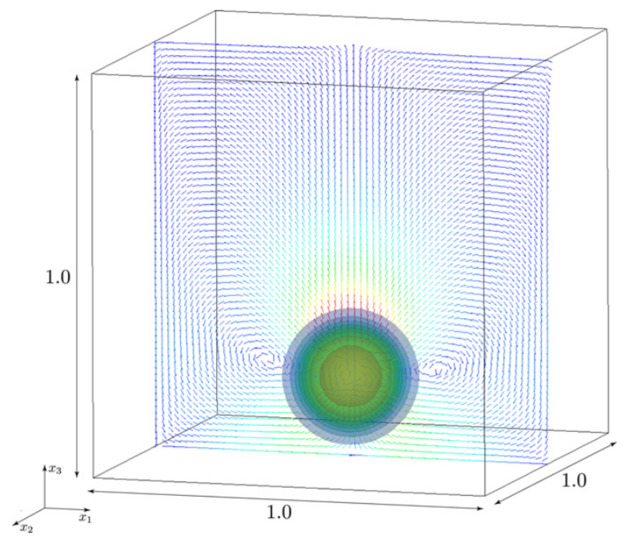
\includegraphics[width=8cm]{images/benchmark_hotblob/fumt11}\\
{\captionfont Simulation setting of BLOB problem. Isosurface and vectors represent temperature field \\and computed flow respectively. Taken from \cite{fumt11}}
\end{center}

%...........................................................
\subsubsection{The punch/indentor problem in 2D} \label{sec:punch}

The punch benchmark is one of the few boundary value problems involving plastic solids for which there exists an exact solution. 
Such solutions are usually either for highly simplified geometries (spherical or axial symmetry, for instance) or simplified material models (such as rigid plastic solids) \cite{kacha04}.

In this experiment, a rigid punch indents a rigid plastic half space; the slip line field theory gives 
exact solutions as shown hereunder:

\begin{center}
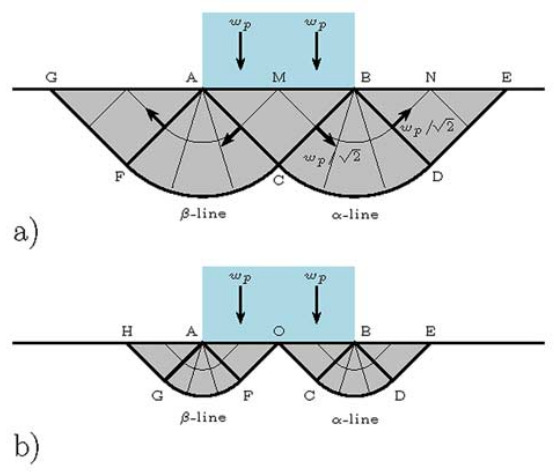
\includegraphics[width=6cm]{images/benchmark_punch/thfb08}\\
{\captionfont Two-dimensional rigid punch indenting a rigid
plastic half space. (a) Prandtl’s rigid plastic solution; (b)
Hill’s solution. Taken from \cite{thfb08}}
\end{center}

The plane strain formulation of the equations and the detailed solution to the problem 
were derived in the Appendix of \cite{thfb08} and are also presented in \cite{gepd98} and in \cite[Chapt.6]{bower2009}.
The two dimensional punch problem has been extensively studied numerically for the past 40 years 
\cite{zihl75,prlo90,zihp95,ziph95,chpe01,chan99,huhy99,yuti06,bufs08,raab07,gltf18} and has been used to draw a parallel with the tectonics of eastern China in the context of the 
India-Eurasia collision \cite{tamo76,mota77,engl82} or the European Alps \cite{repe97}.
It is also worth noting that it has been carried out in one form or another in series of 
analogue modelling articles concerning the same region, with a rigid indenter colliding with a rheologically 
stratified lithosphere \cite{peta88,daco88,jodc90}.
 
Numerically, the one-time step punch experiment is performed on a two-dimensional
domain of purely plastic von Mises material. 
Given that the von Mises rheology yield criterion does not depend on pressure, the density of the material and/or the gravity vector is set to zero. Sides are set to free slip boundary conditions, the bottom to no slip, while a vertical velocity $(0,-v_p)$ is prescribed at the top boundary for nodes whose $x$ coordinate is within $[L_x/2-\delta/2,L_x/2+\delta/2]$. 

The analytical solution predicts that the angle of the shear bands stemming from the sides of the punch 
is $\pi/4$, that the pressure right under the punch is $1+\pi$, 
and that the velocity of the rigid blocks on each side of the punch is $v_p/\sqrt{2}$ 
(this is simply explained by invoking conservation of mass).


\begin{center}
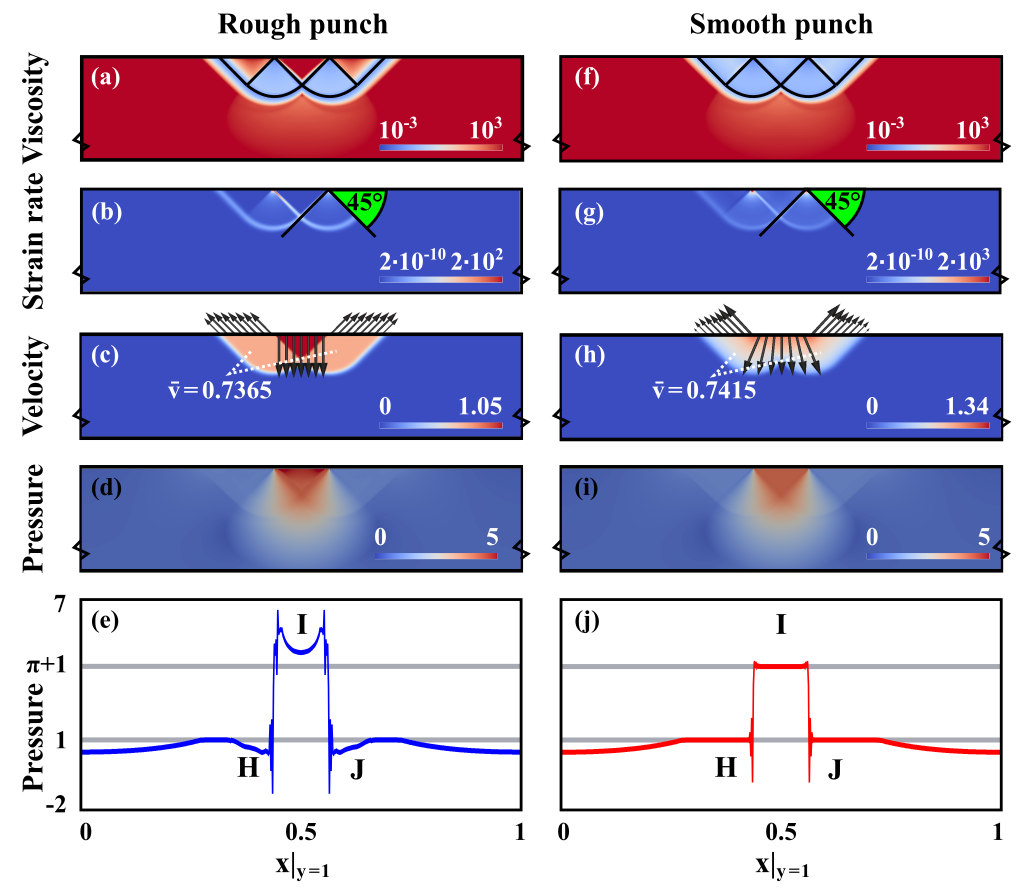
\includegraphics[width=10cm]{images/benchmark_punch/gltf18}\\
{\captionfont The punch benchmark results after 500 nonlinear iterations for a rough punch (left column) 
and a smooth punch (right column). (a,f) Viscosity field with analytical slip lines. 
(b,g) Strain rate norm $\dot\varepsilon_e$ with measured shear band angles. 
(c,h) Velocity magnitude with velocity vectors along the surface of the domain.
(d,i) Pressure field. (e,j) Pressure along the surface of the domain (colored line) and analytical 
solution values $\pi + 1$ and 1 (grey lines). Taken from \cite{gltf18}}
\end{center}

\begin{remark}
This benchmark is often mentioned or used in the context of bearing capacity, footings, 
limit state design/analysis \cite{mich01,zhll03,gour04,gork06,lesk05,shls03}.
\end{remark}


%................................................................................
\subsubsection{Lid driven cavity with analytical solution} \label{sec:ldc_anal}

This comes from \cite{elsw}(section 3.1.4). The velocity is prescribed to be
\[
{\vec v}=(2y(1-x^2) ; -2x(1-y^2) )
\]
with a domain given by $\Omega=[-1:1]\times[-1:1]$.
The strainrate tensor is then given by:
\[
\dot{\bm \varepsilon}=
\left(
\begin{array}{cc}
-4xy & -x^2+y^2  \\
-x^2+y^2 & 4xy   
\end{array}
\right)
\]
The Stokes equation is then:
\begin{eqnarray}
-\frac{\partial p}{\partial x} + 2\eta ( -4y + 2y ) &=& \rho g_x \\
-\frac{\partial p}{\partial y} + 2\eta ( -2x + 4x ) &=& \rho g_y
\end{eqnarray}
where we assume the viscosity $\eta=1$ to be constant in space.
Assuming $g_x=0$, the first equation is
\[
\frac{\partial p}{\partial x} = - 4 y
\]
i.e.
\[
p(x,y)= -4  y x +f(y)
\]
Inserting this in the second equation:
\[
4  x - f'(y) + 4 x  = \rho g_y
\]
or,
\[
-f'(y) + 8  x  = \rho g_y
\]
Assuming $g_y=-1$, we get $\rho=-8x$ and then $f'(y)=0$ so $f(y)=C$ where $C$
is a constant.
Finally the pressure is given by:
\[
p(x,y)=-4  y x + C
\]
We add the following requirement: $\int_\Omega p(x,y) d\Omega =0$ so that $C=0$.

\begin{center}
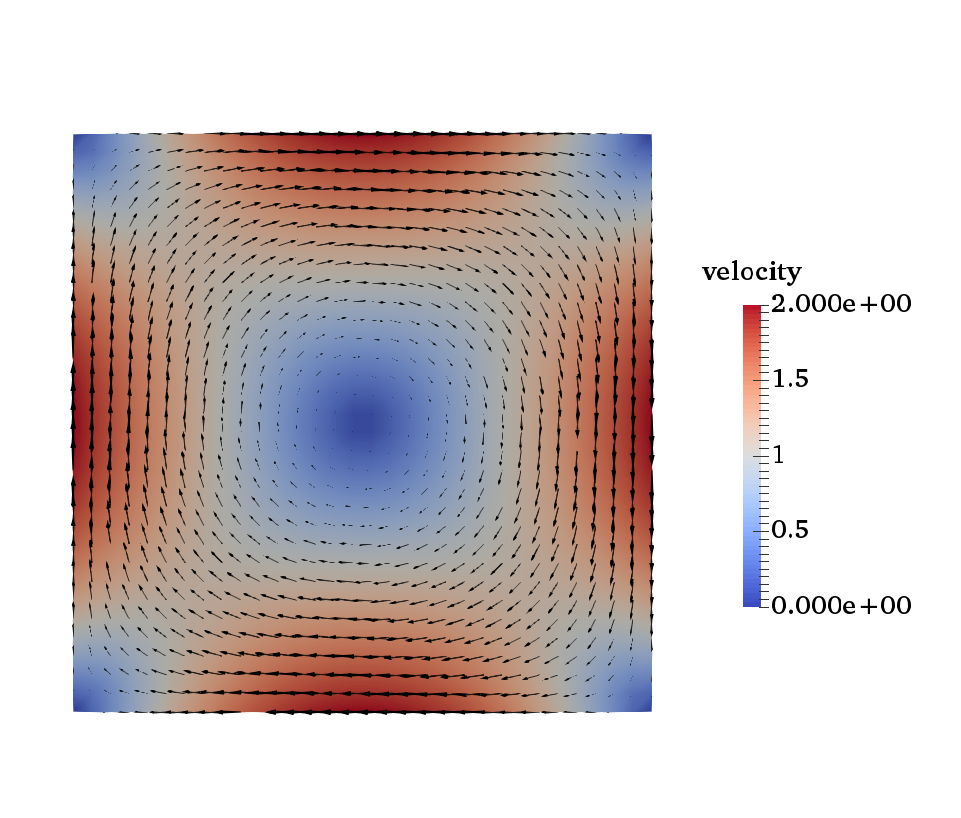
\includegraphics[width=6cm]{images/benchmark_ldc_anal/velo}
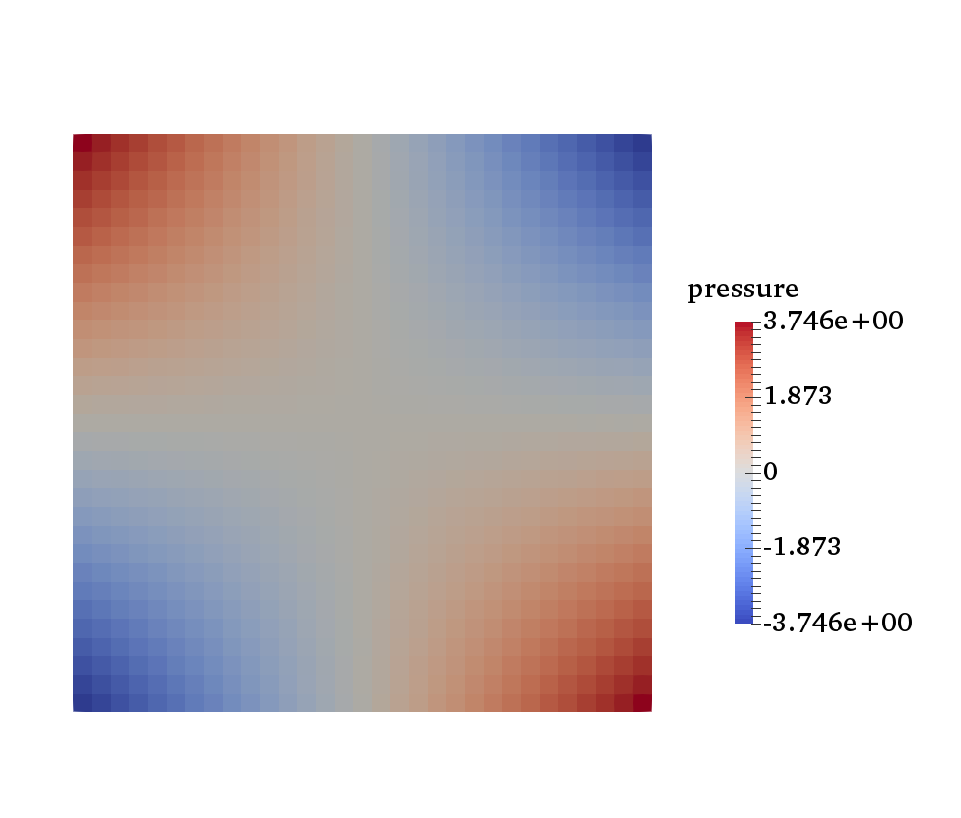
\includegraphics[width=6cm]{images/benchmark_ldc_anal/press}
\end{center}

\begin{eqnarray}
v_{rms}^2 
&=& \frac{1}{\Omega} \int_\Omega (u^2+v^2) d\Omega \nonumber\\
&=& \frac{1}{4} \int_{-1}^{+1}\int_{-1}^{+1} (u^2+v^2) dxdy \nonumber\\
&=& \frac{1}{4} \int_{-1}^{+1}\int_{-1}^{+1} [ 4y^2(1-x^2)^2 + 4x^2(1-y^2)^2   ] dxdy \nonumber\\
&=& 
\end{eqnarray}

\todo[inline]{finish vrms calculation of benchmark}



%................................................................................
\subsubsection{Flow around a cylinder} \ref{sec:flowcyl}

There are many variants of this problem: 2D \cite{turek}, 3D \cite{john02}.
Many studies focus on Navier-Stokes flow since the cylinder generates
vortices at high Reynolds numbers. Steady state solutions at low Re are shown 
here\footnote{\url{up of the test and data measurement}}.
Note the interesting benchmark for 2D visco-elastic flow in \cite{bepo10}.

\begin{center}
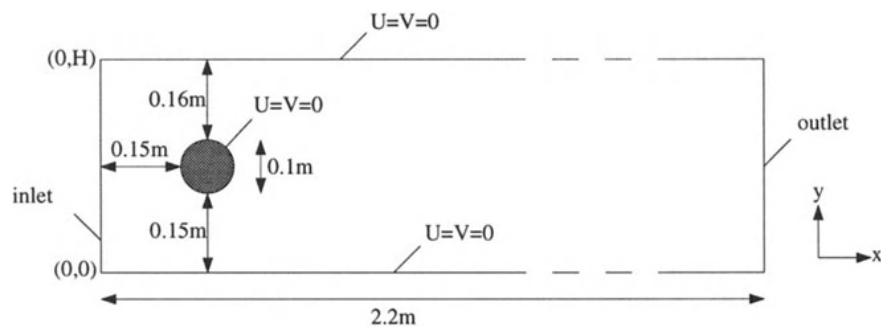
\includegraphics[width=7cm]{images/benchmark_flow_cylinder/turek}
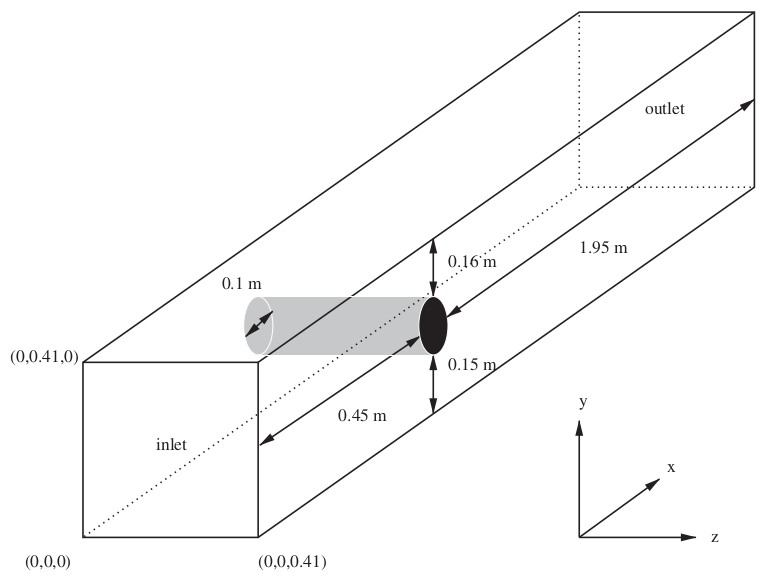
\includegraphics[width=7cm]{images/benchmark_flow_cylinder/john02}\\
{\captionfont Left: taken from \cite{turek}; Right: taken from \cite{john02}}
\end{center}

\Literature: \cite{taie87}

%................................................................................
\subsubsection{Thin layer entrainment} \label{sec:tlentr})
\begin{flushright} {\tiny {\color{gray} benchmark\_thin\_layer\_entrainment.tex}} \end{flushright}

The problem is a simulation to study the
amount of entrainment by thermal convection of a dense,
thin layer at the bottom of the model \cite{vaks97}. 
To the author's knowledge only two other publications \cite{taki03,vant07}
have presented results pertaining to this benchmark.
The results shown here after are obtained with my \elefant code using 
the particle-in-cell technique. 

The box is $2\times 1$, and contains two fluids:
\begin{center}
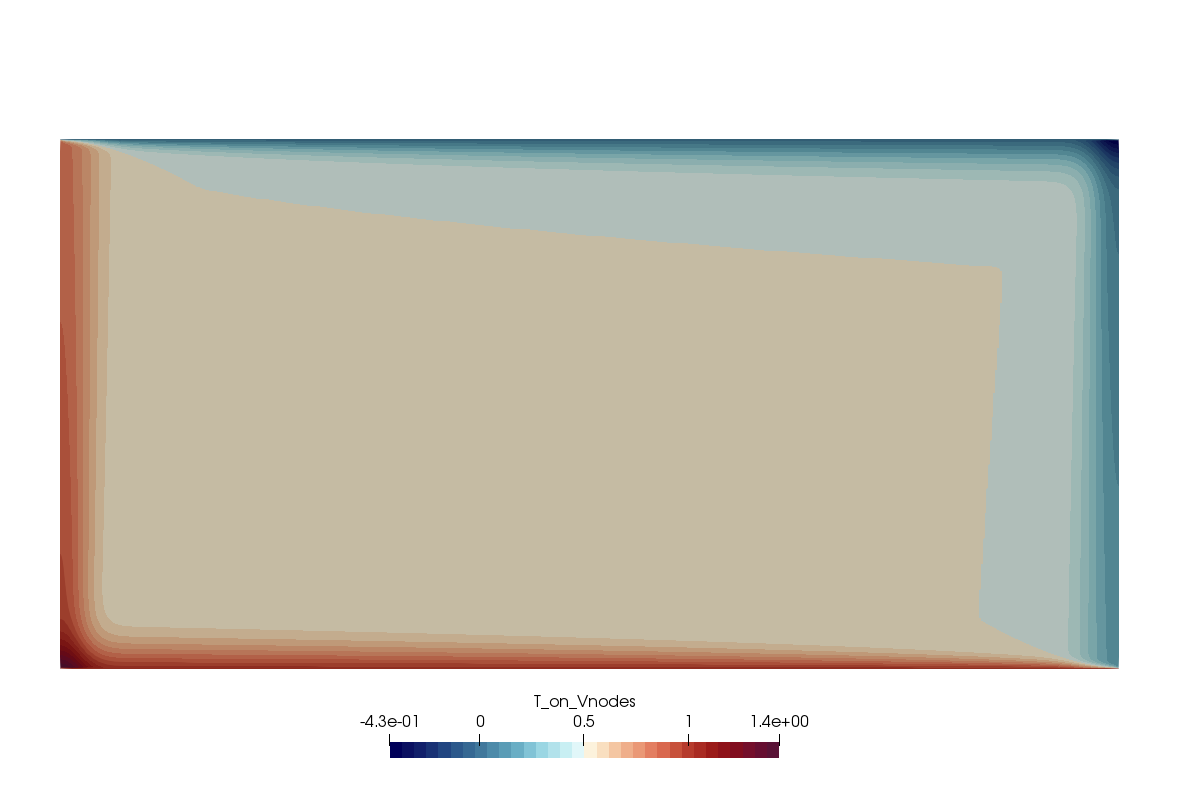
\includegraphics[width=0.45\linewidth]{images/benchmark_thinlayer/temperature_init}
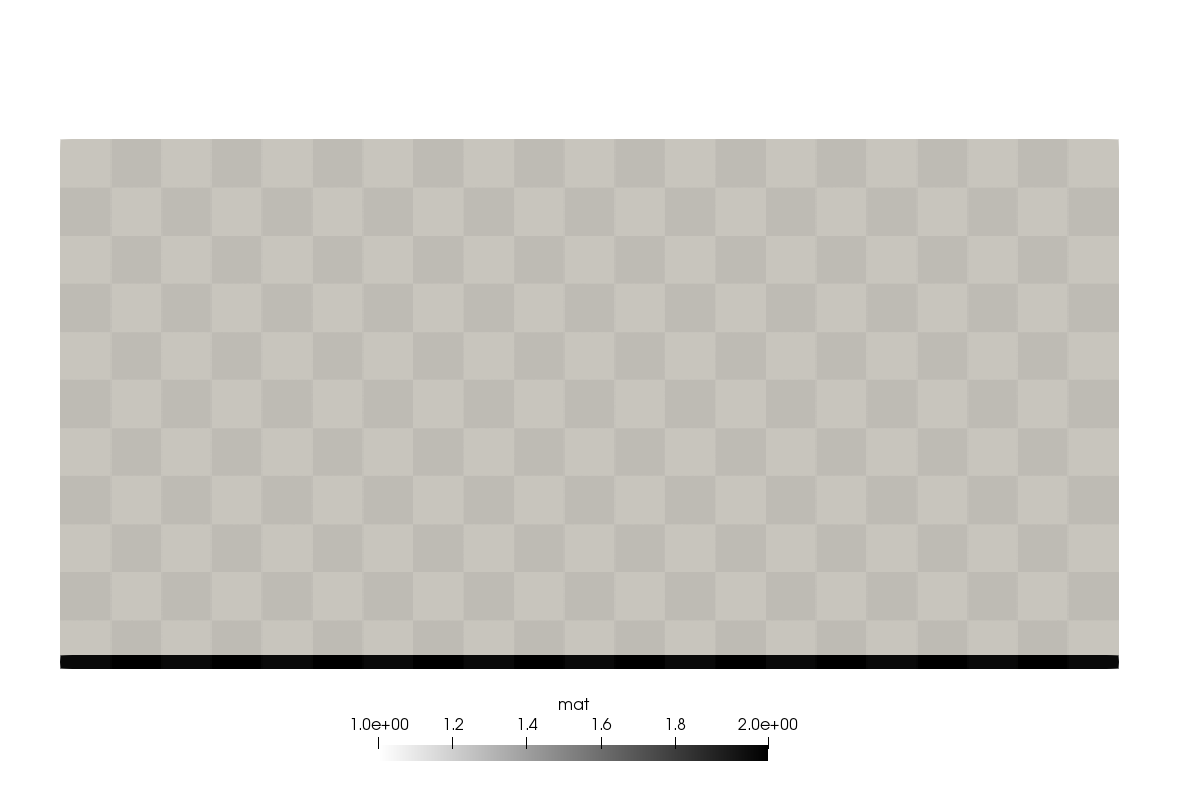
\includegraphics[width=0.45\linewidth]{images/benchmark_thinlayer/mat_init}
\end{center}
Fluid 1 has a density $\rho_1=1$ and a viscosity $\eta=1$.
Fluid 2 is heavier ($\rho_2=\rho_1 + \Delta \rho$) 
but has the same viscosity. 
Both fluids have a thermal expansion coefficient $\alpha=10^{-10}$, a 
thermal conductivity $k=1$, and a heat capacity coefficient $c_p=1$.
Fluid 2 is placed at the bottom of the box ($0\leq y \leq 0.025$).

This experiment is parameterised by the thermal Rayleigh number $Ra=300,000$ and 
and the compositional Rayleigh number $Ra_c=450,000$ which are defined as follows:

\begin{eqnarray}
Ra_T=\frac{\alpha \rho g \Delta T L_y^3}{\kappa \eta}
= \frac{\alpha \rho^2 g \Delta T L_y^3 c_p}{k \eta}
= \alpha g \\
Ra_c&=&\frac{ \Delta \rho g L_y^3}{\kappa \eta}
= \frac{ \rho \Delta \rho g L_y^3 c_p}{k \eta}
= \Delta \rho g
\end{eqnarray}
where I have used the relationship $\kappa=k/\rho c_p$.
$B$ is defined as $B=Ra_T/Ra_c$ so 
The gravity acceleration is therefore set to $g=Ra/\alpha$ and this yields $\Delta \rho=Ra_c/g=B Ra_T/g = B\times \alpha$.

Free-slip boundary conditions are imposed on all sides of the domain.
Temperature boundary conditions are $T(x,y=0)=1$ and 
$T(x,y=1)=0$. The analytical initial temperature field is given by 
\begin{equation}
T(x,y)=T_u(x,y)+T_l(x,y)+T_r(x,y)+T_s(x,y)-\frac{3}{2}
\end{equation}
where
\begin{eqnarray}
T_u(x,y) &=& \frac{1}{2} {\rm erf} \left(  \frac{1-y}{2} \sqrt{\frac{u_0}{x}} \right) \nonumber\\
T_l(x,y) &=& 1-\frac{1}{2} {\rm erf} \left( \frac{y}{2} \sqrt{\frac{u_0}{L_x-x}} \right) \nonumber\\
T_r(x,y) &=& \frac{1}{2} + \frac{Q}{2\sqrt{\pi}} \sqrt{\frac{u_0}{y+1}} \exp \left(  -\frac{x^2u_0}{4y+4} \right) \nonumber\\
T_s(x,y) &=& \frac{1}{2} - \frac{Q}{2\sqrt{\pi}} \sqrt{\frac{u_0}{2-y}} \exp \left(  -\frac{(L_x-x)^2u_0}{8-4y} \right) 
\end{eqnarray}
with
\begin{equation}
u_0=\frac{L_x^{7/3}}{(1+L_x^4)^{2/3}} \left(\frac{Ra}{2\sqrt{\pi}} \right)^{2/3}
\quad\quad
Q=2\sqrt{\frac{L_x}{\pi u_0}}
\end{equation}
Using $L_x=2$, $Ra=3\times10^5$, one gets
$u_0 \simeq 1469.315 $ and $Q\simeq 0.0416305$.

Given the small thickness of the bottom layer, it seems quite legitimate to 
investigate the influence of grid resolution on the simulation. 
I have therefore looked at the initial root mean square velocity measurement 
as a function of the element diagonal value (a proxy for the average resolution
in the case where elements are not square). 


Results are confirm that 
the element size plays a non negligible role at startup on the dynamics of the system.
Superimposed on the figure are the measurements provided by Prof. van Keken (black squares
in the gray box).
They agree well with my measurements but also indicate that 
none of the authors in the original study ran the experiment at a high-enough resolution
to start with (their results were therefore most likely resolution dependent).

We see that the number of markers per element at startup is critical at 
(very) low resolution but that it does not lead to 
significant velocity variations at high resolution. 

\begin{center}
\includegraphics[width=0.65\linewidth]{images/benchmark_thinlayer/thie14}\\
{\scriptsize 
Thin layer entrainment experiment: root mean square velocity measurements at
$t=0$ as a function of the element diagonal size. 
The red square points correspond to resolutions where the number of elements in each direction 
is a multiple of 40 (i.e. $L_y/d$), so that no element would contain a mix of fluids 1 and 2. 
Pink points correspond to cases wherethe number of markers within each element was varied between 4 and 500 
(random spatial distribution). Taken from \cite{thie14}}
\end{center}


Looking at the root mean square velocity measurements, we see that
the measurements done with \elefant agree nicely with those presented in \cite{vaks97}. 
Past $t\sim0.015$, the curves diverge clearly across all codes and authors, 
so I only need to focus the comparison for times $t <0.015$. 
For the three tested resolutions,measurements agree well and fall within the grey curves 
representing all results of van Keken et al. 
Additional tests have been carried out concerning the value of the
Courant number (0.1 to 0.25) and the initial number of markers per element (100 or 200) 
and these parameters led to extremely similar results.

\begin{center}
\includegraphics[width=0.65\linewidth]{images/benchmark_thinlayer/thie14b}\\
{\scriptsize Thin layer entrainment experiment. Root mean square velocity as a function of time.All results presented invan Keken et al.(1997) are collapsed in dashed lines. All simulationswere run with an initial marker density of 100 markers per element and with a Courant numberof 0.25. Taken from \cite{thie14}.}
\end{center}

As observed in van Keken et al., the dense layer is first swept 
into the lower left corner. Thermal instabilities then further develop in an asymmetrical way 
and entrain the dense material. Past $t\simeq 0.015$ the system becomes more 
and more chaotic with markers being randomly mixed in the system in a non-orderly fashion.

\begin{center}
\includegraphics[width=0.23\linewidth]{images/benchmark_thinlayer/maarkers0000}
\includegraphics[width=0.23\linewidth]{images/benchmark_thinlayer/maarkers0025}
\includegraphics[width=0.23\linewidth]{images/benchmark_thinlayer/maarkers0050}
\includegraphics[width=0.23\linewidth]{images/benchmark_thinlayer/maarkers0075}\\
\includegraphics[width=0.23\linewidth]{images/benchmark_thinlayer/maarkers0100}
\includegraphics[width=0.23\linewidth]{images/benchmark_thinlayer/maarkers0125}
\includegraphics[width=0.23\linewidth]{images/benchmark_thinlayer/maarkers0150}
\includegraphics[width=0.23\linewidth]{images/benchmark_thinlayer/maarkers0175}\\
\includegraphics[width=0.23\linewidth]{images/benchmark_thinlayer/maarkers0200}
\includegraphics[width=0.23\linewidth]{images/benchmark_thinlayer/maarkers0225}
\includegraphics[width=0.23\linewidth]{images/benchmark_thinlayer/maarkers0250}
\includegraphics[width=0.23\linewidth]{images/benchmark_thinlayer/maarkers0275}\\
{\scriptsize  marker distribution as obtained with \elefant for 
grid 240x120, init\_marker\_density=7, random distribution, 
CFL=0.25, rkmethod=2, m\_to\_q=2. Unpublished.}
\end{center}


\Literature: Trim \etal (2020) \cite{trlb20}.





%................................................................................
\subsubsection{Heat flow around a cylinder} \label{sec:hfcyl}

The domain is a 2D Cartesian box of size 8x4.
The Stokes equations are not solved and the following velocity is prescribed:
\begin{eqnarray}
u(x,y)&=& U_\infty \left(  1-\frac{x^2-y^2}{(x^2+y^2)^2}  \right) \\
v(x,y)&=& -2U_\infty \frac{xy}{(x^2+y^2)^2}
\end{eqnarray}
Boundary conditions are as follows:
$T=0$ is imposed at the top and bottom of the domain. 
$T=1$ is imposed inside a disc centered at (2,2) with radius 1.  
Further: $k=0.01$, $c_p=1$, $\rho=1$, CFL number is 0.1.

\begin{center}
\includegraphics[width=5cm]{images/benchmark_heatcyl/u}
\includegraphics[width=5cm]{images/benchmark_heatcyl/w}
\includegraphics[width=5cm]{images/benchmark_heatcyl/vel}
\end{center}

\begin{center}
\includegraphics[width=5cm]{images/benchmark_heatcyl/temper_0000}
\includegraphics[width=5cm]{images/benchmark_heatcyl/temper_0020}
\includegraphics[width=5cm]{images/benchmark_heatcyl/temper_0040}\\
\includegraphics[width=5cm]{images/benchmark_heatcyl/temper_0060}
\includegraphics[width=5cm]{images/benchmark_heatcyl/temper_0080}
\includegraphics[width=5cm]{images/benchmark_heatcyl/temper_0150}\\
{\captionfont Time evolution of the temperature field.
Results obtained with ELEFANT (unpublished)}
\end{center}


%................................................................................
\subsubsection{Thermal diffusion of half-cooling space} \label{sec:hcsp}

This is a simple 1D experiment which solution is (for instance) available 
in Turcotte \& Schubert \cite{tusc} and is also presented in \cite{chtl13}.

The domain is 100km deep. $T_0=$0\degree C is prescribed a the surface and 
$T_m=$1300\degree C is prescribed at the bottom. The initial temperature is $T(y)=1300$\degree C.
The material is characterised by $\rho=1000$kg/m$^3$, $C_p=1000$J/kg/K, 
$k=1$J/m/K. The time-dependent solution is given by:
\begin{equation}
T(y,t)=T_0 + (T_0-T_m) \text{erf} \left( \frac{y}{2\sqrt{k t /\rho C_p}}  \right)
\end{equation}

\begin{center}
\includegraphics[width=6cm]{images/benchmark_hcsp/chtl13}\\
{\captionfont Thermal diffusion of half space cooling plate.
The temperature profiles in the analytical solution at 1, 5,
and 15 Myrs are plotted in solid lines. The results from
DynEarthSol2D are plotted in circles. Taken from \cite{chtl13}}
\end{center}


%................................................................................
\subsubsection{Laplace equation on a semi infinite plate} \label{sec:lapplate})
\begin{flushright} {\tiny {\color{gray} benchmark\_laplace\_plate.tex}} \end{flushright}

This experiment is based on a 2nd year mathematics lecture I give at Utrecht University. 
One wishes to solve the Laplace equation for temperature on the following plate subject 
to the indicated boundary conditions:

\begin{center}
\includegraphics[width=3.5cm]{images/benchmark_lapplate/laplace2.png}
\end{center}


The temperature satisfies the 2D Laplace equation inside the plate:
\begin{equation}
\frac{\partial^2 T}{\partial x^2}
+ \frac{\partial^2 T}{\partial y^2} = 0
\end{equation}

We could try to solve the equation by using a tentative solution of the form:
\begin{equation}
T(x,y)=\theta(x) \Phi(y)
\end{equation}

\includegraphics[width=.5cm]{images/benchmark_lapplate/warning.png}
We do not {\it know} the solution is of this form.

We substitute (2) into (1) and obtain:
\[
\Phi \frac{\partial^2 \theta}{\partial x^2} +
\theta \frac{\partial^2 \Phi}{\partial y^2} = 0
\]
Dividing by $\theta\Phi$ gives:
\[
\frac{1}{\theta} \frac{\partial^2 \theta}{\partial x^2} +
\frac{1}{\Phi} \frac{\partial^2 \Phi}{\partial y^2} = 0
\]

Separation of variables: we say that each term is a constant because the first term is a function of $x$ only
and the second a function of $y$ only.
We then write
\[
\frac{1}{\theta} \frac{\partial^2 \theta}{\partial x^2} = - \frac{1}{\Phi} \frac{\partial^2 \Phi}{\partial y^2} = -k^2
\]
where $k$ is called the separation constant.
This leads to 
\[
\frac{\partial^2 \theta}{\partial x^2} + k^2 \theta = 0
\]
\[
\frac{\partial^2 \Phi}{\partial y^2} - k^2 \Phi =0
\]

\begin{itemize}
\item The solution to the first one is $\theta(x)=\sin kx$ or $\theta(x)=\cos kx$
\item The solution to the second one is $\Phi(x)=e^{kx}$ or $\Phi(x)=e^{-kx}$
\end{itemize}


The general solution writes:

\[
T(x,y)=\theta(x) \Phi(y)=
\left\{
\begin{array}{c}
\sin kx \\ \cos kx
\end{array}
\right\}
\left\{
\begin{array}{c}
e^{ky} \\ e^{-ky}
\end{array}
\right\}
\]

We can now use the b.c. to find the solution to the Laplace equation.

\begin{itemize}
\item Since $T\rightarrow 0$ when $y\rightarrow \infty$ then $e^{ky}$ unacceptable.
\item Since $T=0$ when $x=0$ then $\cos kx$ unacceptable.
\end{itemize}

so
\[
T(x,y)=
\sin (kx)  \;
 e^{-kx}
\]

We finally use $T=0$ at $x=10$ which leads to $10k=n \pi$, i.e.:

\[
T(x,y)=\sin (\frac{n\pi x}{10}) \;   e^{-n\pi y/10}
\]

\includegraphics[width=.5cm]{images/benchmark_lapplate/warning.png}
Problem: the solution does not satisfy  $T(x,0)=100$.
However, a linear combination of solutions is still a solution !
Let's find such a combination which satisfies the b.c. at $y=0$ :
\[
T(x,y) = \sum_{n=1}^\infty b_n \sin (\frac{n\pi x}{10}) \;   e^{-n\pi y/10}
\]

We impose then $T(x,0)=100$:
\[
100 = \sum_{n=1}^\infty b_n \sin (\frac{n\pi x}{10}) 
\]
This is the Fourier sine series of $f(x)=100$ with $l=10$ (chapter 7.9 of Boas).

The coefficient $b_n$ is then given by
\[
b_n=\frac{2}{l} \int_0^l f(x) \sin\frac{n \pi x}{l} dx
=\frac{2}{10} \int_0^l 100 \sin\frac{n \pi x}{10} dx
=
\left\{
\begin{array}{ll}
400/n\pi & {\rm odd \; n} \\
0 & {\rm even \; n} \\
\end{array}
\right.
\]

Finally (!):
\[
T(x,y) = 
\frac{400}{\pi}
\left(
e^{-\pi y/10} \sin (\frac{\pi x}{10})
+\frac{1}{3}
\sin (\frac{3\pi x}{10}) \;   e^{-3\pi y/10}
+ \dots
\right)
\]

The simulation has been run with a 10x50 domain. All coefficients of the temperature equation are
set to 1, and the Stokes equation is not solved. The timestep is fixed to $dt=0.1$. Resolution 
is 32x160. 

\begin{center}
a)
\includegraphics[width=1.8cm]{images/benchmark_lapplate/temper0000.png}
\includegraphics[width=1.8cm]{images/benchmark_lapplate/temper0010.png}
\includegraphics[width=1.8cm]{images/benchmark_lapplate/temper0020.png}
\includegraphics[width=1.8cm]{images/benchmark_lapplate/temper0030.png}
\includegraphics[width=1.8cm]{images/benchmark_lapplate/temper0040.png}
\includegraphics[width=1.8cm]{images/benchmark_lapplate/temper0050.png}
\includegraphics[width=1cm]{images/benchmark_lapplate/colourscale.png}
\hspace{.2cm}
b)\includegraphics[width=1.8cm]{images/benchmark_lapplate/temper_analytical.png}\\
{\captionfont a) time evolution of the temperature field; b) analytical steady state solution}
\end{center}







%................................................................................
\subsubsection{Slab detachment benchmark} \label{sec:slabdetach}

\cite{schm11,aspectmanual,gltf18}

\begin{center}
\includegraphics[width=6cm]{images/benchmark_slabdetach/gltf18}\\
{\captionfont The detachment benchmark model setup of Schmalholz \cite{schm11}: 
a symmetric system of nonlinear viscous lithosphere with a vertical slab extending into a linear 
viscous mantle. The top and bottom boundaries are free slip, while the vertical boundaries are no slip.
Taken from \cite{gltf18}.}
\end{center}

%................................................................................
\subsubsection{Layered flow with viscosity contrast} \label{sec:layfl}

The idea behind this benchmark is to construct an analytical solution to the incompressible
Stokes equation in the case where the viscosity field showcases a 
viscosity contrast at location $y=y_0$ whose amplitude and width can be controlled. 
The viscosity is defined as
\[
\eta(y)=\frac{1}{\frac{1}{\pi} \tan^{-1} (\frac{y-y_0}{\beta} ) + 1/2 + \epsilon}
\]
where $\beta$ and $\epsilon$ are parameters. 

\begin{center}
\includegraphics[width=7cm]{images/benchmark_layeredflow/viscosityA}
\includegraphics[width=7cm]{images/benchmark_layeredflow/viscosityB}\\
\includegraphics[width=7cm]{images/benchmark_layeredflow/viscosityC}
\includegraphics[width=7cm]{images/benchmark_layeredflow/viscosityD}\\
{\captionfont Viscosity profiles for different values of $\beta$ and $\epsilon$ 
for $y_0=1/3$.
When $\beta$ is very large, the viscosity 
essentially converges to $\sim (1/2 + \epsilon)^{-1}$. 
$\beta$ controls the width of the transition while $\epsilon$ controls the amplitude 
of the viscosity variation.}
\end{center}

The flow is assumed to take place in an infinitely long pipe (in the horizontal direction)
and bound by 
$y=-1$ and $y+1$.
At the bottom we impose $v_x(y=-1)=0$ while we impose $v_x(y=+1)=1$ at the top.
The density is set to 1 while the gravity is set to zero.
Under these assumptions, the flow velocity and pressure fields are given by:
\begin{eqnarray}
v_x(x,y)&=&\frac{1}{2\pi} \left(  -\beta C_1 \log [\beta^2 + (z-y_0)^2]  + 2 (z-y_0)  C_1 \tan^{-1} \frac{z-y_0}{\beta} + \pi (1+2\epsilon) z C_1  + C_2 \right) \nonumber\\
v_y(x,y) &=& 0 \nonumber\\ 
p(x,y) &=& 0 
\end{eqnarray}
where $C_1$ and $C_2$ are integration constants:
\begin{eqnarray}
C_1 &=& 2\pi \left[ 
 \beta  \log [\beta^2 + (1+y_0)^2]  -  2(1+y_0) \tan^{-1} \frac{1+y_0}{\beta} 
-\beta  \log [\beta^2 + (1-y_0)^2]  +  2(1-y_0) \tan^{-1} \frac{1-y_0}{\beta} + 2\pi (1+2\epsilon)   \right]^{-1} \nonumber\\
C_2 &=&  \left[ \beta  \log [\beta^2 + (1+y_0)^2]  -  2(1+y_0) \tan^{-1} \frac{1+y_0}{\beta} + \pi(1+2\epsilon) \right]C_1, 
\end{eqnarray}

\begin{center}
\includegraphics[width=7cm]{images/benchmark_layeredflow/layeredflow_vel}
\includegraphics[width=7cm]{images/benchmark_layeredflow/layeredflow_viscosity}\\
{\captionfont Velocity and viscosity fields}
\end{center}

\paragraph{Analytical derivations} 
The flow takes place in the horizontal direction and is infinite in the this direction too so that:
\[
\vec\upnu=(u(y),0)
\]
The strain rate tensor is then given by:
\[
\dot{\bm \varepsilon}=
\frac{1}{2}
\left(
\begin{array}{cc}
0 & du/dy \\
du/dy & 0
\end{array}
\right)
\]
The momentum equation then becomes:
\[
{\vec \nabla} \cdot (2 \eta \dot{\bm \epsilon} ) -{\vec \nabla}p 
=
{\vec \nabla} \cdot \left[ \eta(y) 
\left(
\begin{array}{cc}
0 & du/dy \\
du/dy & 0
\end{array}
\right)
\right] -{\vec \nabla}p 
= \rho {\vec g}
\]
On the vertical axis, when the gravity is zero, the equation is automatically verified when the 
pressure is zero.
On the horizontal axis:
\[
\frac{d}{dy} \left(\eta(y) \frac{du}{dy} \right) = 0
\]
Then 
\[
\eta(y) \frac{du}{dy}  = C_1
\]
or,
\[
\frac{du}{dy}  = \frac{C_1}{\eta(y)} = C_1 \left(\frac{1}{\pi} \tan^{-1} \frac{y-y_0}{\beta} 
+ 1/2 + \epsilon\right)
\]
so that the velocity is given by:
\[
u(y) = \frac{1}{\pi} ( y \tan^{-1}((y-y_0)/\beta) - y_0 \tan^{-1}((y-y_0)/beta)  
-0.5* \beta \log (\beta^2 + y^2 - 2 y y_0 +y_0^2) + \pi y (\epsilon +0.5)) 
\]

\[
u(z)=\frac{1}{2\pi} \left(  -\beta C_1 \log [\beta^2 + (z-y_0)^2]  + 2 (z-y_0)  C_1 \tan^{-1} \frac{z-y_0}{\beta} + \pi (1+2\epsilon) z C_1  + C_2 \right)
\]
where $C_1$ and $C_2$ are integration constants.
I wish to impose $u(z=-1)=0$ and $u(z=+1)=1$:
\[
\frac{1}{2\pi} \left(  -\beta C_1 \log [\beta^2 + (-1-y_0)^2]  + 2 (-1-y_0)  C_1 \tan^{-1} \frac{-1-y_0}{\beta} - \pi (1+2\epsilon)  C_1  + C_2 \right) = 0
\]
\[
\frac{1}{2\pi} \left(  -\beta C_1 \log [\beta^2 + (1-y_0)^2]  + 2 (1-y_0)  C_1 \tan^{-1} \frac{1-y_0}{\beta} + \pi (1+2\epsilon)  C_1  + C_2 \right) = 1
\]
or,
\[
 -\beta C_1 \log [\beta^2 + (-1-y_0)^2]  + 2 (-1-y_0)  C_1 \tan^{-1} \frac{-1-y_0}{\beta} - \pi (1+2\epsilon)  C_1  + C_2 = 0
\]
\[
 -\beta C_1 \log [\beta^2 + (1-y_0)^2]  + 2 (1-y_0)  C_1 \tan^{-1} \frac{1-y_0}{\beta} + \pi (1+2\epsilon)  C_1  + C_2 = 2\pi
\]
or,
\[
 -\beta C_1 \log [\beta^2 + (-1-y_0)^2]  + 2 (1+y_0)  C_1 \tan^{-1} \frac{1+y_0}{\beta} - \pi (1+2\epsilon)  C_1  + C_2 = 0
\]
\[
 -\beta C_1 \log [\beta^2 + (1-y_0)^2]  + 2 (1-y_0)  C_1 \tan^{-1} \frac{1-y_0}{\beta} + \pi (1+2\epsilon)  C_1  + C_2 = 2\pi
\]




or,
\[
-\beta C_1 \log (\beta^2 + (1+y_0)^2)  +  2(1+y_0)C_1 \tan^{-1} ((1+y_0)/\beta) - \pi (1+2\epsilon)  C_1  +C_2  = 0
\]
\[
-\beta C_1 \log (\beta^2 + (1-y_0)^2)  +  2(1-y_0)C_1 \tan^{-1} ((1-y_0)/\beta) + \pi (1+2\epsilon)C_1  +C_2  = 2\pi
\]
I can now substract the first line from the second line:
\[
\beta C_1 \log (\beta^2 + (1+y_0)^2)  -  2(1+y_0)C_1 \tan^{-1} ((1+y_0)/\beta)  
-\beta C_1 \log (\beta^2 + (1-y_0)^2)  +  2(1-y_0)C_1 \tan^{-1} ((1-y_0)/\beta) + 2\pi (1+2\epsilon)C_1    = 2\pi
\]
i.e.,
\[
C_1= 2\pi \left[ 
 \beta  \log [\beta^2 + (1+y_0)^2]  -  2(1+y_0) \tan^{-1} [\frac{1+y_0}{\beta}] 
-\beta  \log [\beta^2 + (1-y_0)^2]  +  2(1-y_0) \tan^{-1} [\frac{1-y_0}{\beta}] + 2\pi (1+2\epsilon)   \right]^{-1}
\]
and then 
\[
C_2= \beta C_1 \log (\beta^2 + (1+y_0)^2)  -  2(1+y_0)C_1 \tan^{-1} ((1+y_0)/\beta) + \pi(1+2\epsilon) C_1 
\]



%\newpage

%\newpage
%For $\epsilon=0$

%\begin{center}
%\includegraphics[width=15cm]{viscosityA}\\
%\includegraphics[width=5cm]{velocity1}
%\includegraphics[width=5cm]{velocity3}
%\includegraphics[width=5cm]{velocity5}
%\end{center}

%\newpage
%For $\epsilon=0.1$

%\begin{center}
%\includegraphics[width=15cm]{viscosityB}\\
%\includegraphics[width=5cm]{velocity6}
%\includegraphics[width=5cm]{velocity8}
%\includegraphics[width=5cm]{velocity10}
%\end{center}



%................................................................................
\subsubsection{Elastic material in simple shear} \label{sec:elastsimpshear}

The domain is a Cartesian box of size $1\times1$. The boundary conditions are as follows:
\begin{itemize}
\item bottom: $u=v=0$
\item top: $u=1$, $v=0$
\end{itemize}
The shear modulus $\mu$ is set to 1, and the Poisson ratio $\nu$ is set to 0.25. 
Gravity is set to zero. 

The analytical solution for this problem is given by 
\[
\vec{\upnu}=
\left(
\begin{array}{c}
y \\
0 
\end{array}
\right)
\]
so that 
\[
\vec{\nabla}\vec{\upnu}=
\left(
\begin{array}{cc}
0 & 0 \\
1 & 0
\end{array}
\right)
\quad\quad
{\bm \varepsilon} = 
\frac{1}{2}
\left(
\begin{array}{cc}
0 & 1 \\
1 & 0
\end{array}
\right)
\]
The stress tensor then writes:
\[
{\bm \sigma}= \lambda \vec{\nabla}\cdot \vec{\upnu} + 2 \mu {\bm \varepsilon} 
= \mu 
\left(
\begin{array}{cc}
0 & 1 \\
1 & 0
\end{array}
\right)
\]
since $\vec{\nabla}\cdot \vec{\upnu}=0$.

The principal direction angle $\theta_p$ defines the principal
directions where the only stresses are normal stresses, and 
is given by the relationship:
\[
\tan (2\theta_p) =  \frac{2 \sigma_{xy}}{\sigma_{xx} -\sigma_{yy}}
\]
In our case the rhs is equal to $\infty$, which means that $2 \theta_p = \frac{\pi}{2}$
so that $\theta_p=\frac{\pi}{4}$.

The principal stresses are found from the original stresses via
\[
\sigma_{1,2}=\frac{\sigma_{xx}+\sigma_{yy}}{2} \pm \sqrt{  \left( \left(\frac{\sigma_x-\sigma_y}{2}\right)^2 +\sigma_{xy}^2  \right)}
\]
In our case 
\[
\sigma_{1,2} = \pm \sigma_{xy} = \pm \mu
\]
When plotting the principal stresses on the domain we expect crosses at 45\degree. 


%................................................................................
\subsubsection{Elastic material in pure shear} \label{sec:elastpureshear}

This is the same material as the previous benchmark but the boundary conditions are 
now as follows: $u=-1$ on the left, $u=1$ on the right, $v=1$ on the bottom and $v=-1$
on the top. 

In this case we have 
\[
u(x,y)=2(x-1/2) 
\qquad
v(x,y)=-2(y-1/2) 
\]
so 
\[
\vec{\nabla}\vec{\upnu}=
\left(
\begin{array}{cc}
2 & 0 \\
0 & -2
\end{array}
\right)
={\bm \varepsilon}
\]
and $\vec{\nabla}\cdot \vec{\upnu}=0$ so that 
the stress tensor then writes:
\[
{\bm \sigma}= \lambda \vec{\nabla}\cdot \vec{\upnu} + 2 \mu {\bm \varepsilon} 
= 2\mu 
\left(
\begin{array}{cc}
2 & 0 \\
0 & -2
\end{array}
\right)
\]

The principal direction angle $\theta_p$ defines the principal
directions where the only stresses are normal stresses, and 
is given by the relationship:
\[
\tan (2\theta_p) =  \frac{2 \sigma_{xy}}{\sigma_{xx} -\sigma_{yy}} = 0
\]
which means that $\theta_p = 0$.
Then the principal stresses are found from the original stresses via
\[
\sigma_{1,2}=\frac{\sigma_{xx}+\sigma_{yy}}{2} \pm \sqrt{  \left( \left(\frac{\sigma_x-\sigma_y}{2}\right)^2 +\sigma_{xy}^2  \right)}
\]
In our case 
\[
\sigma_{1,2} = \pm 4 \mu 
\]
When plotting the principal stresses on the domain we expect crosses which align with the axis. 






%................................................................................
\subsubsection{Uniform strip load on elastic material} \label{sec:elaststripload}


%\begin{center}
%\includegraphics[width=8cm]{ELASTOMECHANICS/UNIFORM_STRIP_LOAD/fig2}
%\end{center}

From Davis and Selvadurai \cite{dase96}(section 4.6) we have the components of the stress tensor:
\[
\sigma_{xx}=\frac{p_0}{\pi}\left[ \theta - \frac{1}{2}\sin 2\theta  \right]^{\theta_2}_{\theta_1}
\quad\quad\quad
\sigma_{zz}=\frac{p_0}{\pi}\left[ \theta + \frac{1}{2}\sin 2\theta  \right]^{\theta_2}_{\theta_1}
\quad\quad\quad
\sigma_{xz}=\frac{p_0}{\pi}\left[ \sin^2 \theta  \right]^{\theta_2}_{\theta_1}
\]
or, 
\begin{eqnarray}
\tilde{\sigma}_{xx}&=&\left[ \theta - \frac{1}{2}\sin 2\theta  \right]^{\theta_2}_{\theta_1} = \Theta - \frac{1}{2} ( \sin 2\theta_2 - \sin 2\theta_1) \nn\\
\tilde{\sigma}_{zz}&=&\left[ \theta + \frac{1}{2}\sin 2\theta  \right]^{\theta_2}_{\theta_1} = \Theta + \frac{1}{2} ( \sin 2\theta_2 - \sin 2\theta_1) \nn\\
\tilde{\sigma}_{xz}&=&\left[ \sin^2 \theta  \right]^{\theta_2}_{\theta_1} =  \sin^2 \theta_2 - \sin^2 \theta_1 \nn
\end{eqnarray}
with $\Theta=\theta_2-\theta_1$ and $\tilde{\sigma}_{ij}=\sigma_{ij}\pi/p_0$.
The (dimensionless) principal stresses are given by 
\[
\tilde{\sigma}_{1,2}=\frac{\tilde{\sigma}_{xx}+\tilde{\sigma}_{zz}}{2} \pm \sqrt{  \left(\frac{\tilde{\sigma}_{xx}-\tilde{\sigma}_{zz}}{2}\right)^2 +\tilde{\sigma}_{xz}^2 }
\]
We have
\begin{eqnarray}
\frac{\tilde{\sigma}_{xx}+\tilde{\sigma}_{zz}}{2} &=&  \Theta 
\nn\\
\frac{\tilde{\sigma}_{xx}-\tilde{\sigma}_{zz}}{2}
&=&  -\frac{1}{2} (  \sin 2\theta_2 - \sin 2\theta_1 ) \nn\\
&=&  -\frac{1}{2} ( 2 \cos (\theta_1+\theta_2) \sin \Theta ) \nn\\ 
&=&  -\cos (\theta_1+\theta_2) \sin \Theta  \nn\\ 
\tilde{\sigma}_{xz}
&=&\left[ \sin^2 \theta  \right]^{\theta_2}_{\theta_1}  \nn\\
&=&\sin^2 \theta_2 - \sin^2 \theta_1 \nn\\
&=&\frac{1}{2} (1-\cos \theta_2) - \frac{1}{2} (1-\cos 2\theta_1) \nn\\
&=& -\frac{1}{2} (\cos \theta_2 - \cos 2\theta_1) \nn\\
&=& -\frac{1}{2} ( -2 \sin (\theta_1+\theta_2) \sin(\theta_2-\theta_1) ) \nn\\
&=& \sin (\theta_1+\theta_2) \sin \Theta \nn
\end{eqnarray}
so that the principal stresses are finally given by
\[
\sigma_1 = \frac{p_0}{\pi} ( \Theta + \sin \Theta) 
\quad\quad\quad
\sigma_3 = \frac{p_0}{\pi} ( \Theta - \sin \Theta) 
\]
The principal stresses will be constant on any circle that passes through the edges of the 
strip load. It can also be shown that the direction of $\sigma_1$ points toward the highest 
point of this circle.

%\begin{center}
%\includegraphics[width=8cm]{ELASTOMECHANICS/UNIFORM_STRIP_LOAD/fig3}
%\end{center}


